\documentclass[10pt,a4paper,twocolumn]{article}

\usepackage[a4paper,margin=1.75cm,top=1.7cm,bottom=2.0cm]{geometry}
\usepackage{fontspec}
\usepackage{polyglossia}
\setdefaultlanguage{russian}
\setotherlanguage{english}
\setmainfont{Times New Roman}
\setsansfont{Arial}
\setmonofont{Menlo}
\newfontfamily\cyrillicfont{Times New Roman}
\newfontfamily\cyrillicfontsf{Arial}
\newfontfamily\cyrillicfonttt{Courier New}

\usepackage{microtype}
\usepackage{graphicx}
\usepackage{booktabs}
\usepackage{tabularx}
\usepackage{array}
\usepackage{longtable}
\usepackage{caption}
\usepackage{subcaption}
\usepackage{enumitem}
\usepackage{hyperref}
\usepackage{xcolor}
\usepackage{setspace}
\usepackage{amsmath}
\usepackage{amssymb}
\usepackage{mathtools}
\usepackage{multirow}
\usepackage{placeins}
\usepackage{threeparttable}
\usepackage{siunitx}
\usepackage{dblfloatfix}
\usepackage{balance}

\newcolumntype{L}{>{\raggedright\arraybackslash}X}
\newcolumntype{C}{>{\centering\arraybackslash}X}

\graphicspath{{figures/}{../results/paper_ready/}}
\hypersetup{
  colorlinks=true,
  linkcolor=blue!50!black,
  urlcolor=blue!50!black,
  citecolor=blue!50!black,
  pdftitle={Углублённая доразметка и контролируемые пулы кандидатов в переоценке MS MARCO},
  pdfauthor={Автор}
}

\captionsetup{
  font=footnotesize,
  labelfont=bf,
  justification=raggedright,
  singlelinecheck=false
}
\setstretch{1.04}
\raggedbottom
\setlength{\emergencystretch}{1.5em}
\setlength{\columnsep}{0.72cm}
\setlength{\tabcolsep}{5pt}
\renewcommand{\arraystretch}{1.12}
\sisetup{
  detect-all,
  input-decimal-markers = {.},
  table-number-alignment = center
}
\pagestyle{plain}

\title{\textbf{Углублённая доразметка и контролируемые пулы кандидатов}\\[0.25em]
\large в переоценке моделей ранжирования на коллекции MS MARCO}
\author{}
\date{}

\begin{document}

\twocolumn[
\begin{@twocolumnfalse}
\maketitle
\vspace{-1.2em}
\small
\noindent\textbf{Аннотация.} В статье исследуется, как дополнительная ручная разметка влияет на оценку моделей информационного поиска на коллекции MS MARCO. Эта коллекция широко используется для обучения и проверки современных нейросетевых моделей поиска; её многоязычная версия mMARCO включает русский язык, а русская часть входит в состав бенчмарка RusBEIR. Особенность MS MARCO состоит в том, что для большинства запросов в исходной разметке указан только один явно релевантный фрагмент текста. Такая разметка удобна для массового обучения, но может быть недостаточной для точного сравнения поисковых моделей, поскольку в корпусе могут существовать другие релевантные документы, не попавшие в исходную разметку.

В первой части работы используется ручная подвыборка из 1179 запросов и 33667 пар «запрос-документ». Для неё сравниваются исходная разметка MS MARCO, дополнительная человеческая разметка и метки, полученные моделью-судьей, дообученной на основе MiniLM. Во второй части эта модель-судья применяется к полному набору запросов для построения псевдоразметки: документы называются псевдорелевантными, поскольку их релевантность определена не человеком, а автоматически обученной моделью.

Показано, что дополнительная разметка существенно повышает среднее число релевантных документов на запрос и статистически значимо увеличивает метрику качества ранжирования на первых десяти позициях (NDCG@10) для всех рассматриваемых систем. На ручной подвыборке среднее число релевантных документов возрастает с 1.07 до 17.47, а значения этой метрики увеличиваются, в частности, с 0.597 до 0.877 для BM25 и с 0.708 до 0.975 для модели E5 с переранжированием. Для полного набора показано, что среднее число около 130 псевдорелевантных документов на запрос возникает при предъявлении модели-судье большого объединённого пула кандидатов из первых 200 результатов BM25, E5 и BGE. Следовательно, это число нельзя интерпретировать как самостоятельную характеристику корпуса без описания способа формирования пула кандидатов.

\medskip
\noindent\textbf{Ключевые слова:} информационный поиск, MS MARCO, mMARCO, RusBEIR, релевантностная разметка, дополнительная разметка, псевдоразметка, пул кандидатов, объединение ранжированных списков.

\medskip
{\centering
\textbf{Deep Re-annotation and Controlled Candidate Pools}\par
\vspace{0.15em}
\textbf{in the Re-evaluation of Ranking Models on MS MARCO}\par}

\noindent\textbf{Abstract.} This paper studies how deep manual re-annotation and judge-generated pseudo-qrels change the evaluation of retrieval and reranking models on MS MARCO. The analysis combines a manual subset of 1,179 queries with 33,667 query-document pairs and a recovered full-set protocol built from BM25, E5, and BGE runs. We show that manual re-annotation substantially increases qrels density and yields statistically significant gains in the top-10 ranking-quality metric (NDCG@10) for all considered systems. The MiniLM-based judge provides a reproducible automatic baseline with test AUC 0.907, test F1 0.875, and Cohen's $\kappa = 0.636$ on hold-out data. For the recovered full-set pipeline, we demonstrate that the commonly quoted value of about 130 pseudo-relevant documents per query is determined by candidate-pool size rather than by the corpus alone. Reciprocal rank fusion is competitive on a small controlled pool but degrades monotonically as the candidate pool expands. These results indicate that pseudo-qrels density and fusion gains should be interpreted jointly with the candidate-pooling protocol.

\medskip
\noindent\textbf{Keywords:} information retrieval, MS MARCO, qrels, re-annotation, pseudo-qrels, candidate pooling, reciprocal rank fusion, neural reranking.
\vspace{1.0em}
\end{@twocolumnfalse}
]

\section{Введение}

Для обучения современных нейросетевых моделей информационного поиска требуются большие наборы запросов, документов и оценок релевантности. Такие наборы данных позволяют обучать модели не только находить точные совпадения слов, но и учитывать семантическую близость запроса и документа. Одной из наиболее известных коллекций такого типа является MS MARCO, построенная на основе реальных поисковых запросов Bing и используемая для задач ранжирования фрагментов текста и документов \cite{bajaj2016msmarco}. На основе MS MARCO была создана многоязычная коллекция mMARCO, в которой исходные данные переведены на несколько языков, включая русский \cite{bonifacio2022mmarco}. Русская часть mMARCO используется в RusBEIR \textemdash{} русскоязычном бенчмарке для оценки моделей информационного поиска \cite{2025rusbeir}.

Важная особенность MS MARCO состоит в устройстве исходной разметки. В задаче ранжирования фрагментов текста для большинства запросов указан один положительный пример: фрагмент, который может содержать ответ на вопрос пользователя \cite{msmarco_datasets}. Это практично для создания большой коллекции, потому что полная ручная проверка миллионов фрагментов для сотен тысяч запросов была бы слишком дорогой. Однако такая разметка является неполной: если в корпусе существуют другие подходящие фрагменты, они могут отсутствовать в файлах эталонной разметки. Далее под эталонной разметкой понимаются таблицы вида «запрос-документ-метка релевантности», которые используются при вычислении метрик качества ранжирования.

Неполнота разметки особенно важна при сравнении моделей разных типов. Лексические методы, такие как BM25, опираются на совпадения слов. Нейросетевые модели первичного поиска используют векторные представления запросов и документов. Модели переранжирования дополнительно оценивают уже найденные кандидаты более дорогой попарной моделью. Эти подходы могут находить разные релевантные документы. Поэтому модель может вернуть полезный документ, но получить низкую оценку только потому, что этот документ отсутствует в исходной эталонной разметке. По этой причине переоценка MS MARCO после дополнительной разметки представляет самостоятельный исследовательский интерес.

В данной работе изучаются два уровня переоценки. Во-первых, анализируется ручная подвыборка, на которой доступна дополнительная человеческая разметка. Это позволяет сравнить исходную разметку MS MARCO с более плотной разметкой внутри одного и того же набора документов. Во-вторых, рассматривается полный набор запросов MS MARCO. Для него используется модель-судья: бинарный классификатор, который по паре «запрос-документ» выдаёт числовую оценку релевантности и затем, по заданному порогу, относит документ к релевантным или нерелевантным. Такая модель нужна потому, что вручную доразметить полный набор запросов практически невозможно.

Отдельно анализируется метод объединения рангов по обратным рангам (Reciprocal Rank Fusion, RRF). Это не метод разметки и не модель-судья. RRF объединяет несколько ранжированных списков: документ получает больший итоговый балл, если он находится высоко в выдаче нескольких моделей. В работе RRF используется как дополнительная проверка того, повышает ли простое объединение результатов BM25, E5 и BGE качество итоговой выдачи по сравнению с отдельными системами при одной и той же разметке.

Исследование структурировано вокруг трёх исследовательских вопросов.
\begin{enumerate}[leftmargin=1.8em]
\item \textbf{Вопрос 1.} Как дополнительная ручная разметка меняет плотность эталонной разметки и значения метрик качества поиска?
\item \textbf{Вопрос 2.} Насколько надёжна модель-судья как инструмент автоматической псевдоразметки?
\item \textbf{Вопрос 3.} Как размер объединённого пула кандидатов влияет на число псевдорелевантных документов и на качество выдачи после объединения ранжированных списков методом RRF?
\end{enumerate}

Под размером объединённого пула кандидатов понимается число первых документов, которые берутся из выдачи каждой модели перед объединением. Например, при $K=10$ модель-судья получает объединение первых 10 документов BM25, E5 и BGE, а при $K=200$ \textemdash{} объединение первых 200 документов каждой из этих моделей. Именно из-за такого расширения пула в полном эксперименте появляется среднее значение около 130 псевдорелевантных документов на запрос.

Основные результаты состоят в следующем. На ручной подвыборке дополнительная разметка статистически значимо повышает метрики качества поиска для всех рассматриваемых моделей. Модель-судья на базе MiniLM показывает приемлемое качество бинарной классификации и позволяет построить псевдоразметку для полного набора запросов. На полном наборе MS MARCO показано, что высокая плотность псевдоразметки определяется не только свойствами корпуса, но и способом формирования пула кандидатов. Наконец, RRF даёт выигрыш только при небольшом пуле кандидатов; при расширении пула его преимущество исчезает.

\section{Связанные работы}

Коллекция MS MARCO была предложена как крупномасштабный набор данных, основанный на реальных поисковых запросах, и стала одним из стандартных тестовых стендов для ранжирования текстовых фрагментов \cite{bajaj2016msmarco}. Её многоязычная версия mMARCO была создана машинным переводом исходной коллекции и используется для обучения многоязычных моделей поиска \cite{bonifacio2022mmarco}. Для русского языка важен также бенчмарк RusBEIR, объединяющий переведенные, адаптированные и изначально русскоязычные наборы данных для оценки информационного поиска \cite{2025rusbeir}.

В качестве лексического базового метода в подобных постановках традиционно используется BM25 \textemdash{} вероятностная модель ранжирования, основанная на частотах терминов и нормализации длины документа \cite{robertson2009bm25}. Современные нейросетевые методы первичного поиска строятся на векторных представлениях текстов; в рассматриваемом эксперименте используются E5 \cite{wang2022e5} и BGE/FlagEmbedding \cite{xiao2023cpack}. Для переранжирования широко применяются модели типа cross-encoder, основанные на совместной обработке запроса и документа трансформерной моделью \cite{nogueira2019bert}.

Отдельное направление связано с объединением нескольких ранжированных списков. Метод объединения рангов по обратным рангам был предложен как простой способ объединять выдачи разных поисковых систем без обучения дополнительных параметров \cite{cormack2009rrf}. В более поздних работах по гибридному поиску и поиску с генерацией ответов было показано, что RRF остаётся распространенным и практически полезным приемом, но его эффект зависит от состава объединяемых систем, глубины списков и параметров объединения \cite{bruch2023fusion, mackenzie2023anserini, rackauckas2024ragfusion}.

Наша работа не вводит новую поисковую модель. Её вклад состоит в переоценке уже известных моделей после дополнительной разметки, в анализе автоматической псевдоразметки с помощью модели-судьи и в явном разделении двух факторов: качества модели-судьи и размера объединённого пула кандидатов.

\section{Данные и формирование оценочного набора}

\subsection{Исходная коллекция}

Исходным материалом является коллекция MS MARCO Passage Ranking. Она содержит запросы пользователей, корпус из 8841823 коротких текстовых фрагментов и файлы эталонной разметки, в которых для запроса указаны документы, считающиеся релевантными. В исходном файле qrels для dev-части содержится 7437 положительных пар для 6980 запросов, тогда как полный набор запросов, используемый в расширенном протоколе этой работы, содержит 101093 запроса.

Проблема исходной разметки состоит не в том, что указанные положительные документы неверны, а в том, что они часто не исчерпывают все подходящие ответы в корпусе. Например, если запрос спрашивает, к какому округу относится некоторый населённый пункт или объект, в корпусе может быть несколько фрагментов, прямо называющих один и тот же округ. Исходная разметка может содержать только один из них. В таком случае поисковая система, которая вернула другой корректный фрагмент, получает заниженную оценку, потому что этот фрагмент отсутствует в эталонном файле.

\subsection{Формирование ручной подвыборки}

Чтобы исследовать проблему недоразметки, для выбранных запросов был выполнен поиск несколькими системами разных типов. В эксперимент включены лексический поиск BM25, нейросетевые модели первичного поиска E5 и BGE, а также E5 с последующим переранжированием. Для каждого запроса из выдачи каждой системы брались первые 10 документов, после чего эти списки объединялись в один пул кандидатов. Повторяющиеся документы удалялись, поэтому фактическое число документов на запрос обычно было меньше суммы четырёх списков.

Затем документы из объединённого пула были дополнительно размечены человеком. Такая процедура позволяет сравнить три состояния одного и того же оценочного материала: исходную разметку MS MARCO, расширенную человеческую разметку и автоматическую разметку, которую позднее строит модель-судья.

\subsection{Характеристики нового датасета}

Полученная ручная подвыборка содержит 1179 запросов и 33667 пар «запрос-документ». В среднем на один запрос приходится 28.56 документа. В исходной разметке MS MARCO внутри этой подвыборки содержится 1257 положительных пар, то есть в среднем 1.07 релевантного документа на запрос. После дополнительной человеческой разметки число положительных пар возрастает до 20597, то есть до 17.47 релевантного документа на запрос. Таким образом, новый оценочный набор не заменяет MS MARCO, а показывает, насколько сильно меняется плотность разметки внутри специально сформированного пула кандидатов.

В дальнейшем эта ручная подвыборка используется для двух задач. Во-первых, на ней сравниваются значения метрик качества поиска при исходной и дополнительной разметке. Во-вторых, она служит обучающим и проверочным материалом для модели-судьи, которая затем применяется к более крупному набору запросов.

\section{Постановка задачи и экспериментальный протокол}

Пусть $\mathcal{Q}$ \textemdash{} множество запросов, $\mathcal{D}$ \textemdash{} корпус документов, а $\mathcal{M}$ \textemdash{} множество ранжирующих систем. Для запроса $q \in \mathcal{Q}$ и модели $m \in \mathcal{M}$ обозначим через $\mathrm{TopK}_m(q)$ множество первых $K$ документов в выдаче модели $m$. Тогда объединённый пул кандидатов определяется как
\begin{equation}
\label{eq:pool}
P_q^{(K)} = \bigcup_{m \in \mathcal{M}} \mathrm{TopK}_m(q).
\end{equation}

Параметр $K$ задаёт, сколько документов берётся из выдачи каждой отдельной системы: при $K=10$ используются первые 10 документов, при $K=200$ \textemdash{} первые 200 документов. После объединения и удаления повторов итоговый пул может содержать меньше чем $K \cdot |\mathcal{M}|$ документов.

На ручной подвыборке множество $\mathcal{M}_{\text{ручн}}$ включает BM25, E5, BGE и E5 с переранжированием. В постановке для полного набора запросов доступно только $\mathcal{M}_{\text{полн}} = \{\text{BM25}, \text{E5}, \text{BGE}\}$. Причина техническая: для BM25, E5 и BGE сохранены полные ранжированные списки результатов, а для E5 с переранжированием такой список для всех запросов в доступных результатах эксперимента отсутствует. Поэтому E5 с переранжированием используется только в ручной части, где все необходимые пары «запрос-документ» уже размечены.

\subsection{Модель-судья}

Модель-судья построена на базе \texttt{cross-encoder/ms-marco-MiniLM-L-6-v2}. Такая архитектура выбрана как компактная и воспроизводимая модель попарной оценки релевантности, уже обученная на MS MARCO и пригодная для дообучения на ручной разметке. Она нужна не как новая поисковая система, а как инструмент масштабирования разметки: модель получает пару «запрос-документ» и возвращает численную оценку релевантности.

Дообучение выполнялось на ручной подвыборке из 1179 запросов и 33667 пар. Разбиение на обучающую, валидационную и тестовую части проводилось по идентификаторам запросов в пропорции 70/15/15 с фиксированным случайным зерном 42: 23543 пары для 825 запросов вошли в обучение, 5122 пары для 177 запросов \textemdash{} в валидационную часть, 5002 пары для 177 запросов \textemdash{} в тестовую часть. Все документы одного запроса попадали только в одну часть. Это исключает утечку данных между обучением, подбором порога и итоговой проверкой. Порог бинаризации выбирался на валидационной части и в финальной конфигурации составил $\tau = -0.2187$.

Пусть $s_\theta(q,d)$ \textemdash{} численная оценка модели-судьи для пары «запрос-документ», а $\tau$ \textemdash{} порог бинаризации. Тогда решение модели-судьи задаётся выражением
\begin{equation}
\label{eq:judge}
\hat y_{\theta,\tau}(q,d) = \mathbb{I}\left[s_\theta(q,d) \ge \tau\right].
\end{equation}

Соответствующее множество псевдорелевантных документов внутри пула $P_q^{(K)}$ равно
\begin{equation}
\label{eq:positive-set}
R_q^{(K)} = \left\{ d \in P_q^{(K)} \; \middle| \; \hat y_{\theta,\tau}(q,d) = 1 \right\},
\end{equation}
а плотность положительных меток определяется как
\begin{equation}
\label{eq:density}
\rho_q^{(K)} = \frac{|R_q^{(K)}|}{|P_q^{(K)}|}.
\end{equation}

\subsection{Протокол для полного набора запросов}

Для полного набора запросов использовались сохранённые ранжированные списки BM25, E5 и BGE. Для каждого размера пула $K \in \{10, 30, 50, 100, 200\}$ из первых $K$ результатов каждой системы строился объединённый пул \eqref{eq:pool}. Затем модель-судья оценивала все пары «запрос-документ» из этого пула и по порогу $\tau$ формировала псевдоразметку. Поэтому результаты полного протокола зависят не только от модели-судьи, но и от того, сколько кандидатов было предъявлено ей на оценку.

\begin{figure*}[t]
\centering
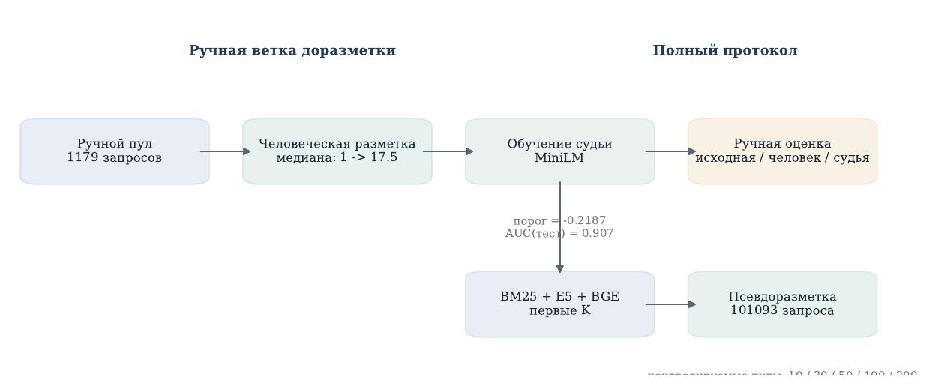
\includegraphics[width=0.92\textwidth]{protocol_schematic.pdf}
\caption{Схема экспериментального протокола. Верхняя ветка соответствует ручной доразметке и обучению модели-судьи, нижняя ветка \textemdash{} протоколу для полного набора запросов с контролируемыми пулами кандидатов. Рисунок подчёркивает, что выводы по ручной подвыборке и по полному набору относятся к различным, хотя и связанным, постановкам.}
\label{fig:protocol}
\end{figure*}

\begin{table*}[t]
\centering
\caption{Сводка экспериментальных постановок и плотности оценочного материала.}
\label{tab:protocol}
\footnotesize
\begin{threeparttable}
\begin{tabularx}{\textwidth}{L C L C C L}
\toprule
\textbf{Постановка} & \textbf{Запросы} & \textbf{Пул} & \textbf{Док./запрос} & \textbf{Рел./запрос} & \textbf{Примеч.} \\
\midrule
Ручная, исходная & 1179 & объединение первых 10 результатов BM25, E5, BGE, E5 с переранжированием & 28.56 & 1.07 & исходная разметка \\
Ручная, дополненная & 1179 & тот же пул & 28.56 & 17.47 & ручная доразметка \\
Полная, псевдоразметка при $K=200$ & 101093 & объединение первых 200 результатов BM25, E5, BGE & 451.54 & 128.64 & все запросы; 130.70 для запросов с непустой выдачей \\
\bottomrule
\end{tabularx}
\begin{tablenotes}[flushleft]
\footnotesize
\item Таблица подчёркивает, что ручная и полная постановки предъявляют на оценку разное число документов. Рост числа релевантных документов в полной постановке обусловлен не только моделью-судьей, но и существенно большим объединённым пулом кандидатов.
\end{tablenotes}
\end{threeparttable}
\end{table*}

Таблица~\ref{tab:protocol} подчёркивает принципиальное различие между ручной и полной постановками. На ручной подвыборке плотность эталонной разметки повышается внутри относительно небольшого пула документов. На полном наборе модель-судья получает существенно больший пул, поэтому высокая плотность псевдоразметки не может интерпретироваться вне контекста выбранного $K$.

\section{Метрики и проверка значимости}

Основной целевой метрикой в работе выступает NDCG@10, то есть нормализованная дисконтированная накопленная полезность на первых десяти позициях выдачи. Для запроса $q$ она рассчитывается через
\begin{align}
\label{eq:dcg}
\mathrm{DCG}@10(q) &= \sum_{i=1}^{10} \frac{2^{\mathrm{rel}_i(q)} - 1}{\log_2(i + 1)}, \\
\label{eq:ndcg}
\mathrm{NDCG}@10(q) &= \frac{\mathrm{DCG}@10(q)}{\mathrm{IDCG}@10(q)}.
\end{align}

Для объединения ранжированных списков используется классический метод RRF:
\begin{equation}
\label{eq:rrf}
\mathrm{RRF}(d \mid q) = \sum_{m \in \mathcal{M}} \frac{1}{c + \mathrm{rank}_m(d,q)}, \qquad c = 60.
\end{equation}

Попарные сравнения выполняются на уровне запросов с помощью парного перестановочного теста. Для двух систем $A$ и $B$ вводится разность
\begin{equation}
\label{eq:delta}
\Delta_q = \mathrm{NDCG}_A(q) - \mathrm{NDCG}_B(q),
\end{equation}
а наблюдаемая статистика имеет вид
\begin{equation}
\label{eq:perm}
T = \frac{1}{|\mathcal{Q}'|} \sum_{q \in \mathcal{Q}'} \Delta_q,
\end{equation}
где $\mathcal{Q}'$ \textemdash{} множество запросов, для которых обе системы имеют корректную оценку. При перестановочном тесте знаки $\Delta_q$ случайно инвертируются, а $p$-значение оценивается как доля перестановок, для которых модуль полученной статистики не меньше наблюдаемого.

Такая постановка важна по двум причинам. Во-первых, она проверяет различия между системами на уровне запросов, а не только по средним. Во-вторых, она позволяет корректно интерпретировать небольшие, но устойчивые отличия, например выигрыш RRF над E5 на узком пуле полного протокола.

\section{Результаты углублённой доразметки}

\subsection{Сдвиг плотности эталонной разметки}

Первый центральный результат состоит в том, что углублённая доразметка радикально меняет плотность эталонной разметки. На ручной части среднее число релевантных документов на запрос возрастает с 1.07 до 17.47, а медиана \textemdash{} с 1 до 17.5. Для автоматической разметки, полученной моделью-судьей на ручной подвыборке, медиана дополнительно возрастает до 19. На псевдоразметке полного набора медиана достигает 93, а 99-й процентиль \textemdash{} 401.

\begin{figure}[t]
\centering
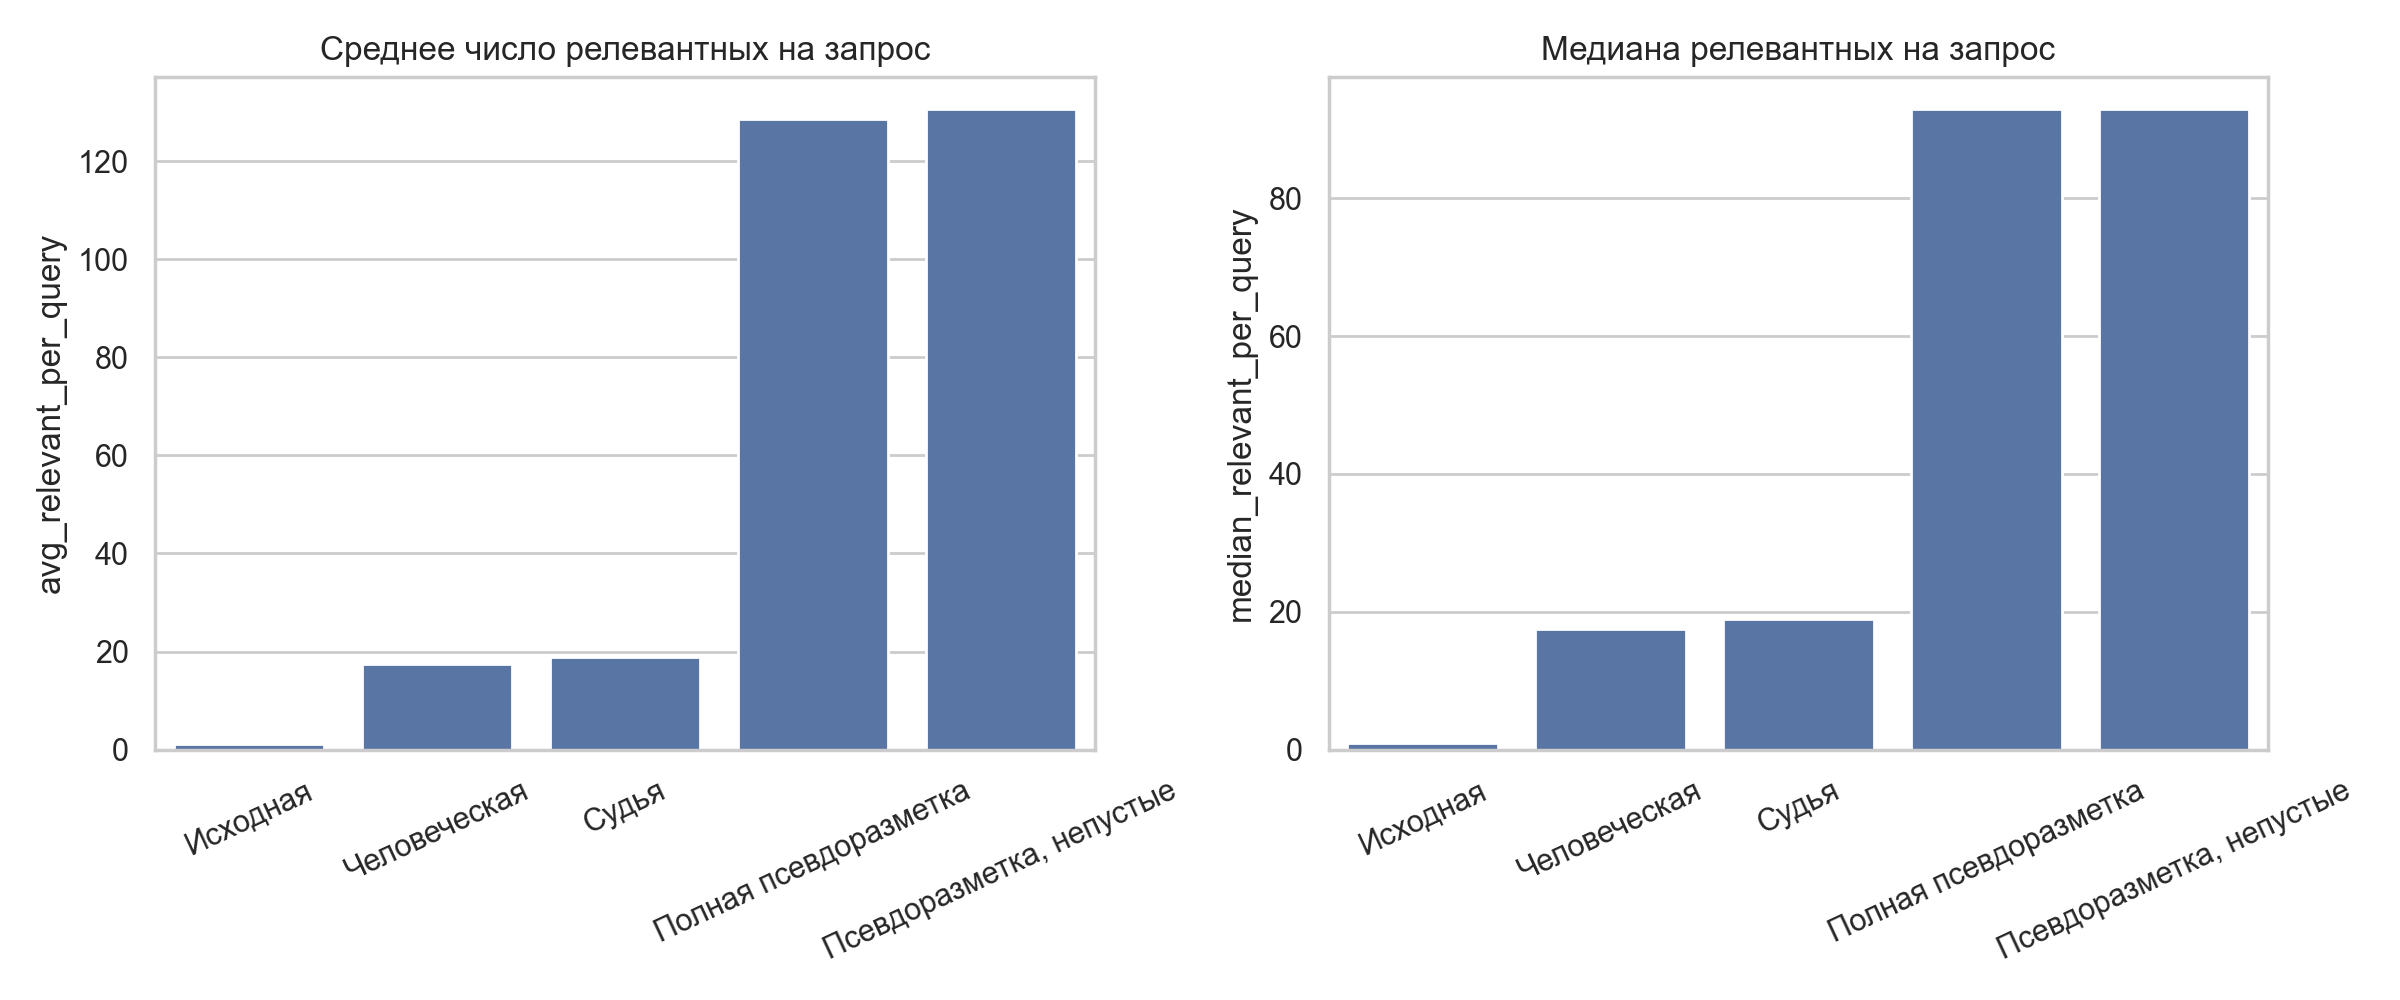
\includegraphics[width=\columnwidth]{qrels_density_comparison.png}
\caption{Сдвиг плотности эталонной разметки между исходной разметкой, дополнительной человеческой разметкой, автоматической разметкой модели-судьи на ручной подвыборке и псевдоразметкой полного набора. Рисунок поддерживает вывод о том, что высокие значения на полном наборе определяются не только свойствами корпуса, но и размером объединённого пула кандидатов.}
\label{fig:density}
\end{figure}

Рисунок~\ref{fig:density} показывает, что число порядка 130 псевдорелевантных документов на запрос не следует интерпретировать как прямую оценку «истинной» релевантности корпуса. Это число возникает в полном протоколе при $K=200$, где средний размер пула составляет 451.54 документа на запрос. Следовательно, наблюдаемая плотность связана как с качеством модели-судьи, так и с протоколом предъявления кандидатов.

\subsection{Изменение качества ранжирования}

На ручной подвыборке углублённая доразметка статистически значимо повышает NDCG@10 для всех базовых моделей. Это относится как к лексическому базовому методу, так и к нейросетевому первичному поиску и переранжированию. Автоматическая разметка, полученная моделью-судьей на ручной части, дополнительно увеличивает значения метрики, однако для интерпретации этих результатов важно отличать её от человеческих меток, поскольку она уже включает ошибку автоматической модели.

\begin{figure}[t]
\centering
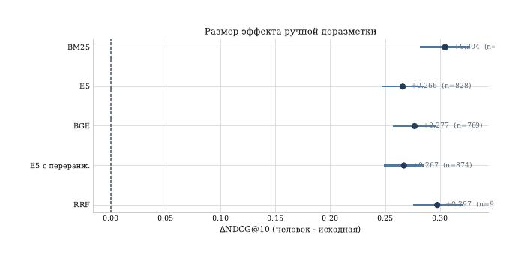
\includegraphics[width=\columnwidth]{manual_effect_forest.pdf}
\caption{Оценки размера эффекта для перехода от исходной разметки к дополнительной человеческой разметке. Точки показывают средний прирост NDCG@10 на уровне запросов, отрезки соответствуют 95\% доверительным интервалам, полученным бутстрэпом.}
\label{fig:effect-forest}
\end{figure}

\begin{table}[t]
\centering
\caption{Парные оценки размера эффекта на уровне запросов для перехода от исходной разметки к дополнительной человеческой разметке.}
\label{tab:effect-ci}
\footnotesize
\begin{tabularx}{\columnwidth}{Lccc}
\toprule
\textbf{Модель} & \textbf{$\Delta$NDCG@10} & \textbf{95\% ДИ} & \textbf{Число запросов} \\
\midrule
BM25 & +0.304 & [0.281; 0.328] & 499 \\
E5 & +0.266 & [0.247; 0.286] & 828 \\
BGE & +0.277 & [0.257; 0.296] & 769 \\
E5 с переранжированием & +0.267 & [0.249; 0.285] & 874 \\
RRF & +0.297 & [0.275; 0.320] & 952 \\
\bottomrule
\end{tabularx}
\end{table}

\noindent Значения в таблице~\ref{tab:effect-ci} рассчитаны как средние парные различия на тех запросах, где для соответствующей модели определены обе оценки. Поэтому они могут немного отличаться от простой разности средних значений в таблице~\ref{tab:main}, где для каждого столбца используется весь доступный набор запросов.

\begin{table*}[t]
\centering
\caption{Основные результаты для ручной подвыборки и полного протокола с объединением первых 10 результатов.}
\label{tab:main}
\footnotesize
\begin{threeparttable}
\begin{tabular}{l S[table-format=1.3] S[table-format=1.3] S[table-format=1.3] S[table-format=1.3] l}
\toprule
\textbf{Модель} & \textbf{Исходная} & \textbf{Человеческая} & \textbf{Судья} & \textbf{Псевдо, полный набор} & \textbf{Примеч.} \\
\midrule
BM25 & 0.597 & 0.877 & 0.908 & 0.642 & лексический базовый метод \\
E5 & 0.701 & 0.967 & 0.979 & 0.855 & нейросетевой первичный поиск \\
BGE & 0.672 & 0.948 & 0.967 & 0.837 & нейросетевой первичный поиск \\
E5 с переранжированием & 0.708 & 0.975 & 0.987 & \multicolumn{1}{c}{\textemdash{}} & нет полного ранжированного списка \\
RRF & 0.607 & 0.906 & \multicolumn{1}{c}{\textemdash{}} & 0.881 & полный протокол для трёх систем \\
\bottomrule
\end{tabular}
\begin{tablenotes}[flushleft]
\footnotesize
\item Значения в столбце «Псевдо, полный набор» для RRF относятся к конфигурации BM25 + E5 + BGE.
\item Полный ранжированный список для E5 с переранжированием среди доступных результатов эксперимента отсутствует, поэтому четырёхсистемное сравнение на полном наборе сознательно не заявляется.
\end{tablenotes}
\end{threeparttable}
\end{table*}

Из таблиц~\ref{tab:main} и \ref{tab:effect-ci}, а также рисунка~\ref{fig:effect-forest} следует, что рост при переходе от исходной к дополнительной человеческой разметке носит систематический характер. В парном расчёте на общих запросах для BM25 прирост составляет $+0.304$, для E5 \textemdash{} $+0.266$, для BGE \textemdash{} $+0.277$, для E5 с переранжированием \textemdash{} $+0.267$, для RRF \textemdash{} $+0.297$. Во всех перечисленных случаях парный перестановочный тест даёт $p < 0.001$, а 95\% доверительные интервалы прироста на уровне запросов не пересекают нулевую линию.

Важно также, что на ручной подвыборке RRF не становится лучшей системой. На дополнительной человеческой разметке E5 с переранжированием достигает 0.975 и остаётся сильнейшей доступной моделью, тогда как RRF даёт 0.906. Это означает, что углублённая доразметка не приводит к автоматическому усилению любых методов объединения ранжированных списков.

\subsection{Качество модели-судьи}

Модель-судья на базе MiniLM выступает не как финальная сильнейшая архитектура, а как воспроизводимый базовый инструмент для автоматической оценки релевантности. Несмотря на сравнительно лёгкую основу модели, качество судьи оказывается достаточным для анализа полного набора запросов.

\begin{figure*}[t]
\centering
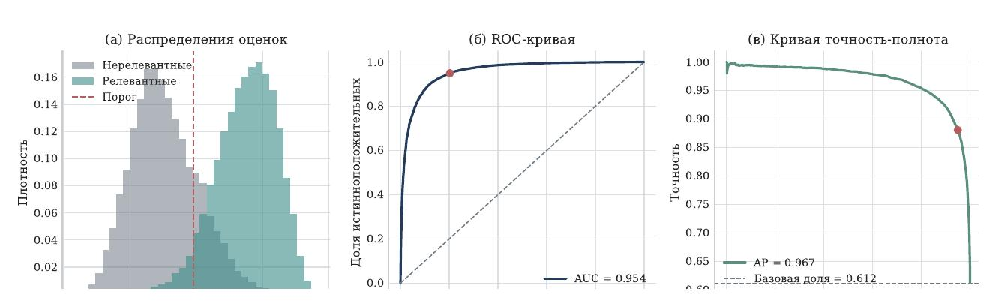
\includegraphics[width=0.95\textwidth]{judge_score_diagnostics.pdf}
\caption{Диагностика численных оценок модели-судьи на аннотированной ручной части. Показаны распределения оценок для релевантных и нерелевантных пар, ROC-кривая и кривая точность-полнота; красной точкой отмечено положение выбранного порога. Эта визуальная диагностика дополняет независимые метрики на отложенной выборке, но не заменяет их.}
\label{fig:judge}
\end{figure*}

Согласно независимой оценке на отложенной выборке, модель-судья достигает площади под ROC-кривой (AUC) 0.908 на валидационной части и 0.907 на тестовой части, F1 0.875 на тестовой части и коэффициента согласия Коэна $\kappa = 0.636$ на отложенной выборке. Дополнительно модель покрывает 95.05\% ручных релевантных пар и даёт точность 87.97\% относительно человеческих меток. Рисунок~\ref{fig:judge} показывает, что даже на уровне численных оценок наблюдается хорошее разделение положительных и отрицательных пар; это делает MiniLM-судью достаточным базовым инструментом для первой статьи, хотя не исключает последующего сравнения с более мощными моделями переранжирования.

\begin{figure*}[t]
\centering
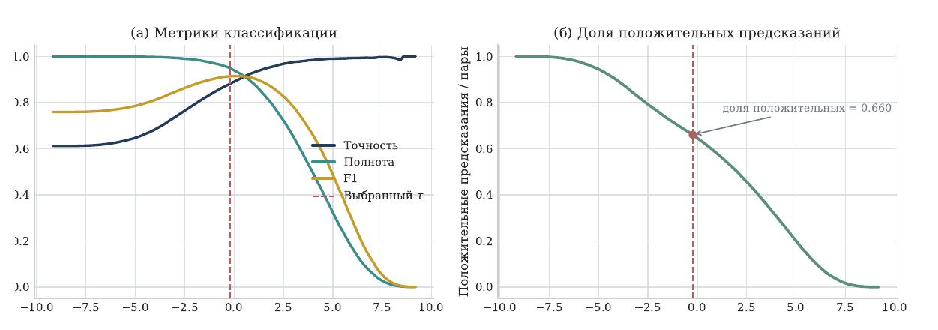
\includegraphics[width=0.90\textwidth]{judge_threshold_sensitivity.pdf}
\caption{Чувствительность модели-судьи к выбору порога $\tau$ на аннотированной ручной части. Слева показаны точность, полнота и F1, справа \textemdash{} доля пар, отнесённых моделью к релевантным. Вертикальная линия соответствует выбранному рабочему порогу $\tau = -0.2187$.}
\label{fig:judge-threshold}
\end{figure*}

Рисунок~\ref{fig:judge-threshold} позволяет содержательно интерпретировать выбранный рабочий порог. На аннотированной ручной части порог $\tau = -0.2187$ соответствует точности $0.881$, полноте $0.949$, F1 $0.914$ и доле предсказанных релевантных пар $0.660$. Эти значения не следует смешивать с метриками обобщающей способности на отложенной выборке: они характеризуют именно положение рабочего порога на размеченном пуле кандидатов и помогают понять, почему модель-судья генерирует достаточно плотную псевдоразметку.

\section{Псевдоразметка полного набора и контролируемые пулы}

Постановка для полного набора показывает, что свойства псевдоразметки необходимо анализировать совместно с глубиной объединённого пула кандидатов. Для $K=10$ среднее число кандидатов на запрос равно 21.88, а среднее число документов, отнесённых моделью-судьей к релевантным, \textemdash{} 14.19. Для $K=200$ эти значения увеличиваются до 451.54 и 128.64 соответственно, тогда как доля положительных меток снижается с 0.649 до 0.285.

\begin{figure*}[t]
\centering
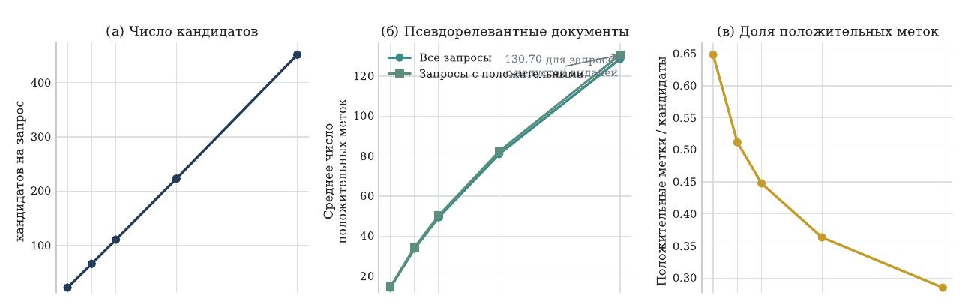
\includegraphics[width=0.94\textwidth]{pool_scaling_multipanel.pdf}
\caption{Изменение свойств псевдоразметки полного набора при увеличении размера объединённого пула кандидатов. Рисунок показывает, что рост числа псевдорелевантных документов следует рассматривать одновременно с ростом числа предъявленных кандидатов и с падением доли положительных меток.}
\label{fig:pool-scaling}
\end{figure*}

\begin{figure*}[t]
\centering
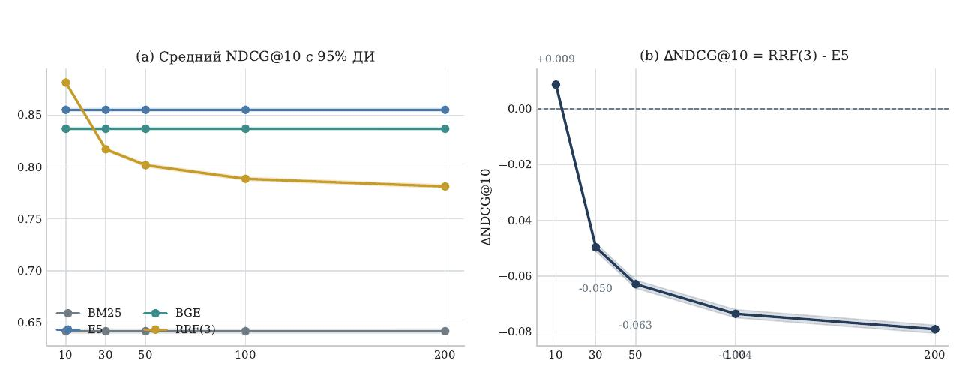
\includegraphics[width=0.94\textwidth]{fullset_uncertainty_panels.pdf}
\caption{Оценка неопределённости в полном протоколе. Слева показаны средние значения NDCG@10 с 95\% доверительными интервалами, полученными бутстрэпом, для BM25, E5, BGE и RRF(3) при различных размерах объединённого пула кандидатов. Справа приведена разность $\Delta$NDCG@10 между RRF(3) и E5, демонстрирующая смену знака при переходе от пула первых 10 результатов к более крупным пулам.}
\label{fig:fullset-uncertainty}
\end{figure*}

Рисунки~\ref{fig:pool-scaling} и \ref{fig:fullset-uncertainty} отражают главный вывод полной части. На узком пуле при $K=10$ RRF даёт лучший результат среди доступных конфигураций полного протокола: 0.881 против 0.855 у E5 и 0.837 у BGE. Однако при увеличении $K$ качество RRF монотонно снижается: 0.817 для $K=30$, 0.802 для $K=50$, 0.789 для $K=100$ и 0.781 для $K=200$. Правая панель рисунка~\ref{fig:fullset-uncertainty} показывает, что разность «RRF минус E5» имеет положительный знак только при $K=10$ ($\Delta = +0.0087$, 95\% доверительный интервал $[0.0075; 0.0098]$), тогда как уже при $K=30$ становится отрицательной и далее лишь увеличивается по модулю. Следовательно, рост плотности эталонной разметки не эквивалентен росту качества ранжирования, а тезис о силе метода объединения оказывается чувствителен к протоколу отбора кандидатов.

\begin{table}[t]
\centering
\caption{Ключевые попарные сравнения, подтверждающие основные выводы статьи.}
\label{tab:sig}
\scriptsize
\setlength{\tabcolsep}{3pt}
\begin{tabularx}{\columnwidth}{@{}L c c c@{}}
\toprule
\textbf{Сравнение} & \textbf{$\Delta$ NDCG@10} & \textbf{$p$-значение} & \textbf{Число запросов} \\
\midrule
RRF на человеческой разметке против BM25 & +0.0372 & $< 0.001$ & 1102 \\
RRF на человеческой разметке против E5 & -0.0582 & $< 0.001$ & 1171 \\
RRF на человеческой разметке против E5 с переранжированием & -0.0680 & $< 0.001$ & 1175 \\
RRF при $K=10$ против E5 & +0.0087 & $< 0.001$ & 95517 \\
RRF при $K=200$ против E5 & -0.0791 & $< 0.001$ & 98527 \\
\bottomrule
\end{tabularx}
\end{table}

Таблица~\ref{tab:sig} подтверждает два связанных вывода. Во-первых, на дополнительной человеческой разметке RRF статистически уступает E5 с переранжированием. Во-вторых, на псевдоразметке полного набора знак преимущества RRF над E5 меняется при переходе от $K=10$ к $K=200$. Следовательно, тезис о «силе» метода объединения зависит от протокола отбора кандидатов и не может переноситься между постановками без дополнительных оговорок.

\section{Угрозы валидности и обсуждение}

Полученные результаты требуют аккуратной интерпретации с точки зрения валидности экспериментальной постановки.

\paragraph{Конструктивная валидность.} Углублённая доразметка меняет не только абсолютные значения метрик, но и саму сравнительную картину между моделями. Это означает, что разреженная эталонная разметка в MS MARCO может существенно занижать качество сильных моделей первичного поиска и переранжирования. Вместе с тем и человеческая разметка, и псевдоразметка зависят от того, какие документы были предъявлены на оценку.

\paragraph{Валидность протокола.} Псевдоразметку высокой плотности на полном наборе нельзя обсуждать в отрыве от размера объединённого пула кандидатов. Число порядка 130 положительных оценок на запрос является свойством конкретного полного протокола, а не «естественной» характеристикой корпуса MS MARCO. Именно поэтому в статье используется анализ контролируемых пулов, а не единичное число без оговорок.

\paragraph{Валидность модели-судьи.} Анализ модели-судьи в основной части использует два типа свидетельств: метрики классификации на отложенной выборке и диагностику численных оценок на аннотированной ручной части. Эти свидетельства взаимодополняют друг друга, но не эквивалентны: ROC-кривая, кривая точность-полнота и анализ чувствительности к порогу характеризуют рабочее поведение судьи на доступной разметке, тогда как AUC и F1 на отложенной выборке отражают его обобщающую способность.

\paragraph{Внешняя валидность.} Полная часть статьи ограничена конфигурацией из трёх систем: BM25, E5 и BGE. Поскольку полный ранжированный список E5 с переранжированием для всех запросов не найден, мы сознательно не формулируем выводы для четырёхсистемного объединения на полном корпусе. Кроме того, все выводы относятся к коллекции MS MARCO и к конкретному протоколу отбора кандидатов; перенос их на другие корпуса требует отдельной проверки.

\paragraph{Практическое обсуждение.} Несмотря на эти ограничения, результаты дают устойчивый вывод по всем трём исследовательским вопросам. Для \textbf{вопроса 1} показано, что углублённая доразметка статистически повышает NDCG@10 и меняет плотность эталонной разметки. Для \textbf{вопроса 2} показано, что модель-судья на базе MiniLM имеет достаточное качество для базовой автоматической псевдоразметки, но требует контроля порога и проверки на отложенной выборке. Для \textbf{вопроса 3} установлено, что интерпретация числа 130.7 неотделима от размера объединённого пула кандидатов, а RRF полезен только в пределах небольшого контролируемого пула и не является универсально сильным методом объединения.

\section{Заключение}

В статье показано, что углублённая доразметка на MS MARCO приводит к существенному изменению плотности эталонной разметки и к статистически значимому росту NDCG@10 для всех рассмотренных систем. На ручной подвыборке E5 с переранжированием остаётся сильнейшей моделью, а модель-судья на базе MiniLM обеспечивает достаточно точный базовый инструмент для автоматической генерации псевдоразметки.

Для полного протокола установлено, что размер объединённого пула кандидатов является ключевым фактором интерпретации результатов. При небольшом объединённом пуле RRF даёт лучший результат среди доступных конфигураций, однако при расширении пула кандидатов его качество монотонно снижается. Следовательно, показатели плотности псевдоразметки и выигрыша методов объединения должны анализироваться не изолированно, а вместе с протоколом отбора кандидатов.

Практический вывод состоит в том, что псевдоразметка на полном корпусе полезна как исследовательский инструмент, но требует анализа контролируемых пулов и явных ограничений в формулировке выводов. В этом смысле переоценка MS MARCO должна обсуждаться не только как улучшение разметки, но и как уточнение самого протокола измерения качества.

\clearpage
\begin{thebibliography}{99}

\bibitem{bajaj2016msmarco}
P.~Bajaj, D.~Campos, N.~Craswell, L.~Deng, J.~Gao, X.~Liu, R.~Majumder, A.~McNamara, B.~Mitra, T.~Nguyen, M.~Rosenberg, X.~Song, A.~Stoica, S.~Tiwary, T.~Wang.
\newblock \textit{MS MARCO: A Human Generated MAchine Reading COmprehension Dataset}.
\newblock arXiv preprint arXiv:1611.09268, 2016.

\bibitem{msmarco_datasets}
Microsoft.
\newblock \textit{MS MARCO datasets}.
\newblock \url{https://microsoft.github.io/msmarco/}, accessed 2026.

\bibitem{bonifacio2022mmarco}
L.~Bonifacio, V.~Jeronymo, H.~Queiroz Abonizio, I.~Campiotti, M.~Fadaee, R.~Lotufo, R.~Nogueira.
\newblock \textit{mMARCO: A Multilingual Version of MS MARCO Passage Ranking Dataset}.
\newblock arXiv preprint arXiv:2108.13897, 2021.

\bibitem{2025rusbeir}
G.~, M.~Tikhomirov, E.~Kozhevnikov, M.~Kornilov, N.~.
\newblock \textit{Building Russian Benchmark for Evaluation of Information Retrieval Models}.
\newblock Computational Linguistics and Intellectual Technologies, 2025.

\bibitem{robertson2009bm25}
S.~E. Robertson, H.~Zaragoza.
\newblock \textit{The Probabilistic Relevance Framework: BM25 and Beyond}.
\newblock Foundations and Trends in Information Retrieval, 3(4):333\textendash{}389, 2009.

\bibitem{wang2022e5}
L.~Wang, N.~Yang, X.~Huang, B.~Jiao, L.~Yang, D.~Jiang, R.~Majumder, F.~Wei.
\newblock \textit{Text Embeddings by Weakly-Supervised Contrastive Pre-training}.
\newblock arXiv preprint arXiv:2212.03533, 2022.

\bibitem{xiao2023cpack}
S.~Xiao, Z.~Liu, P.~Zhang, N.~Muennighoff, D.~Lian, J.-Y. Nie.
\newblock \textit{C-Pack: Packed Resources for General Chinese Embeddings}.
\newblock arXiv preprint arXiv:2309.07597, 2023.

\bibitem{nogueira2019bert}
R.~Nogueira, K.~Cho.
\newblock \textit{Passage Re-ranking with BERT}.
\newblock arXiv preprint arXiv:1901.04085, 2019.

\bibitem{cormack2009rrf}
G.~V. Cormack, C.~L.~A. Clarke, S.~B{\"u}ttcher.
\newblock \textit{Reciprocal Rank Fusion outperforms Condorcet and Individual Rank Learning Methods}.
\newblock In \textit{Proceedings of the 32nd Annual International ACM SIGIR Conference on Research and Development in Information Retrieval}, pp.~758\textendash{}759, 2009.

\bibitem{bruch2023fusion}
S.~Bruch, S.~Gai, A.~Ingber.
\newblock \textit{An Analysis of Fusion Functions for Hybrid Retrieval}.
\newblock arXiv preprint arXiv:2210.11934, 2022.

\bibitem{mackenzie2023anserini}
X.~Ma, T.~Teofili, J.~Lin.
\newblock \textit{Anserini Gets Dense Retrieval: Integration of Lucene's HNSW Indexes}.
\newblock In \textit{Proceedings of the 32nd ACM International Conference on Information and Knowledge Management}, 2023.

\bibitem{rackauckas2024ragfusion}
Z.~Rackauckas.
\newblock \textit{RAG-Fusion: A New Take on Retrieval-Augmented Generation}.
\newblock International Journal on Natural Language Computing, 13(1), 2024.

\end{thebibliography}

\clearpage
\onecolumn
\appendix
\section{Дополнительные материалы}

\begin{figure}[htbp]
\centering
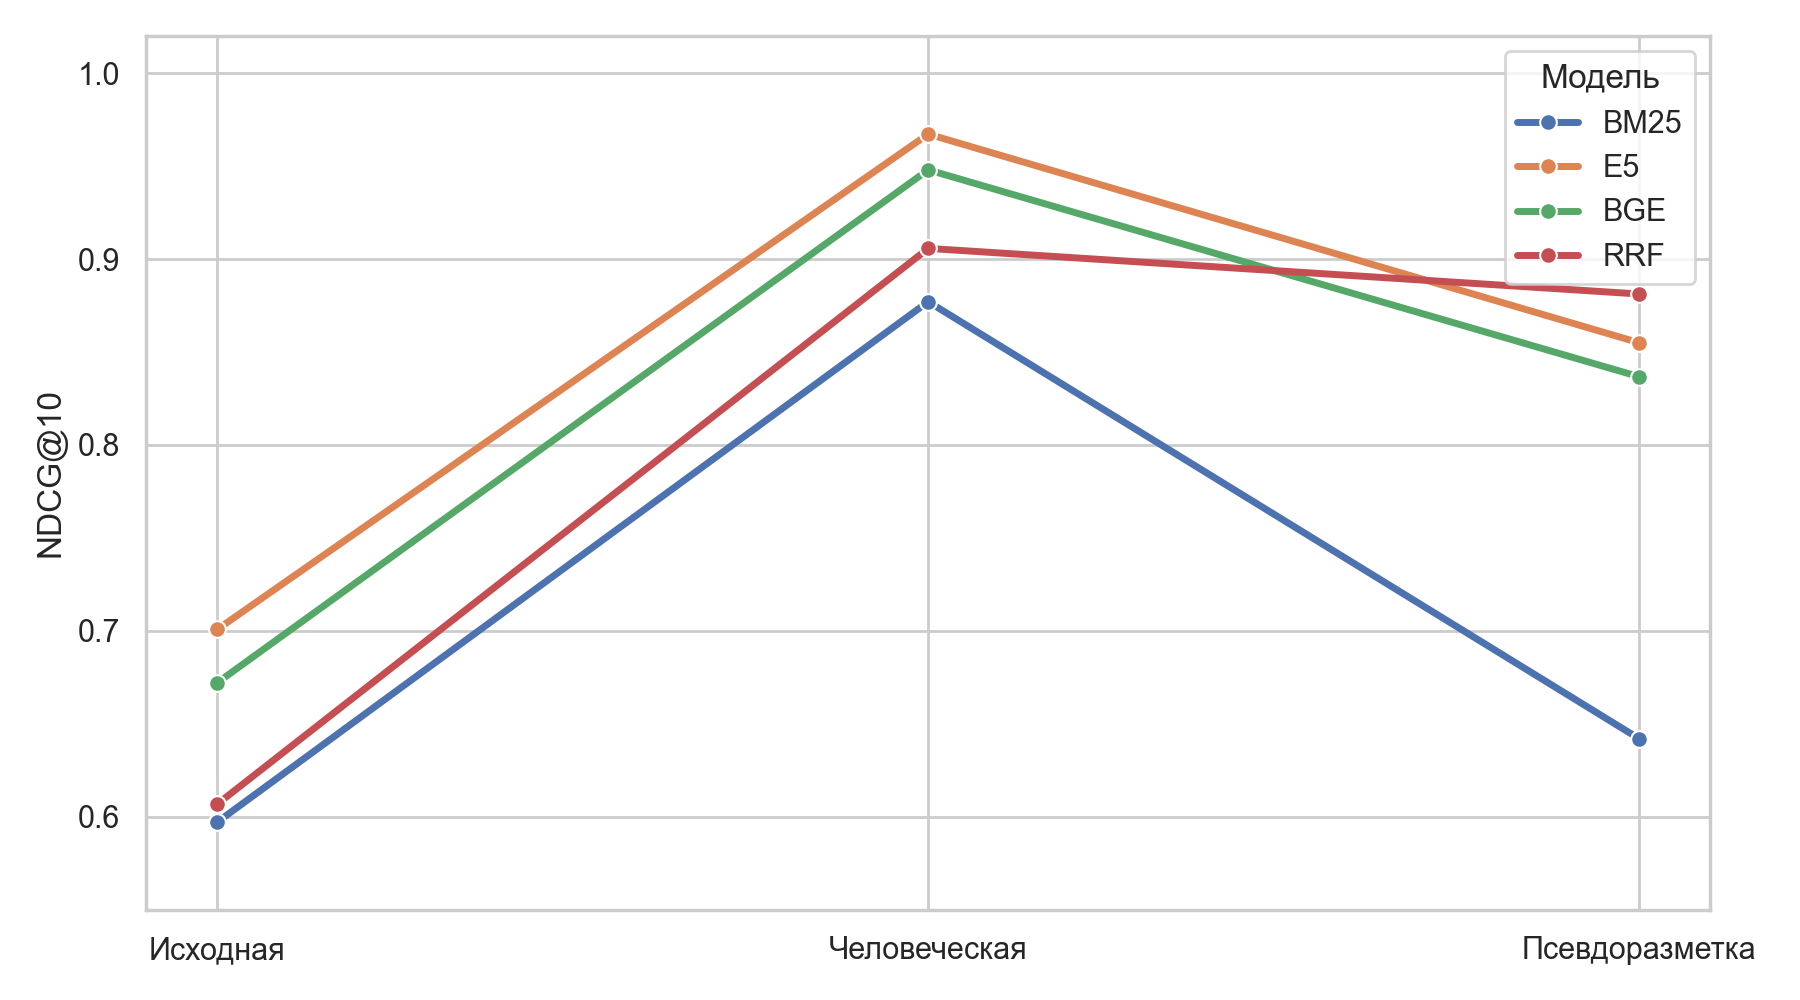
\includegraphics[width=0.90\textwidth]{claim_storyline.png}
\caption{Траектории изменения NDCG@10 при переходе от исходной разметки к дополнительной человеческой разметке и псевдоразметке полного набора.}
\label{fig:app-story}
\end{figure}

\begin{figure}[htbp]
\centering
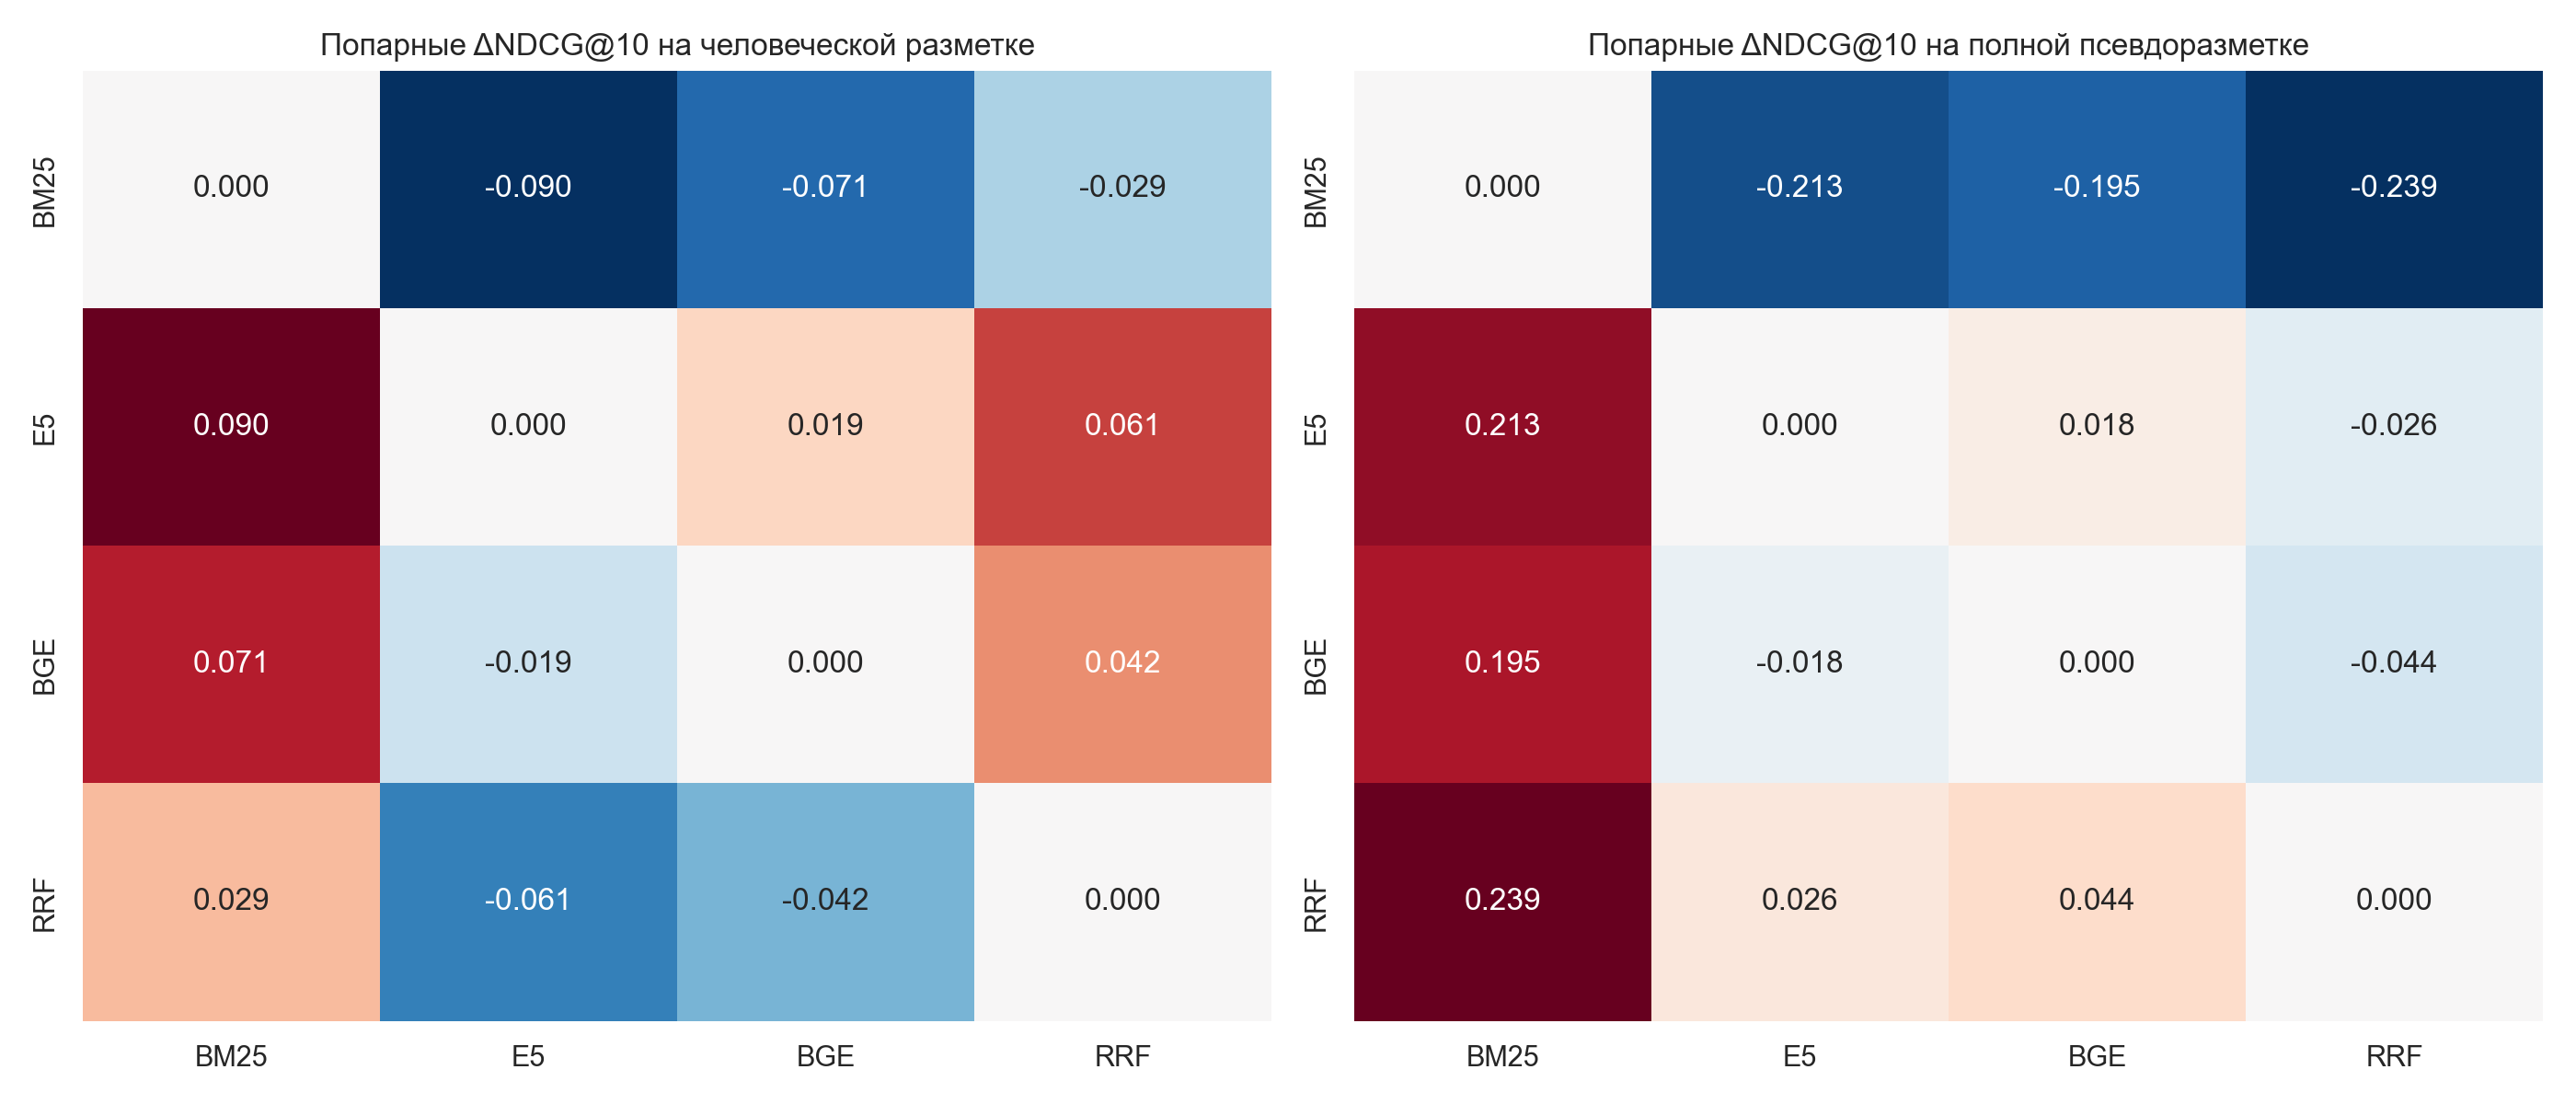
\includegraphics[width=0.94\textwidth]{pairwise_delta_heatmaps.png}
\caption{Попарные различия по NDCG@10: слева \textemdash{} дополнительная человеческая разметка, справа \textemdash{} псевдоразметка полного набора при $K=10$.}
\label{fig:app-heat}
\end{figure}

\begin{figure}[htbp]
\centering
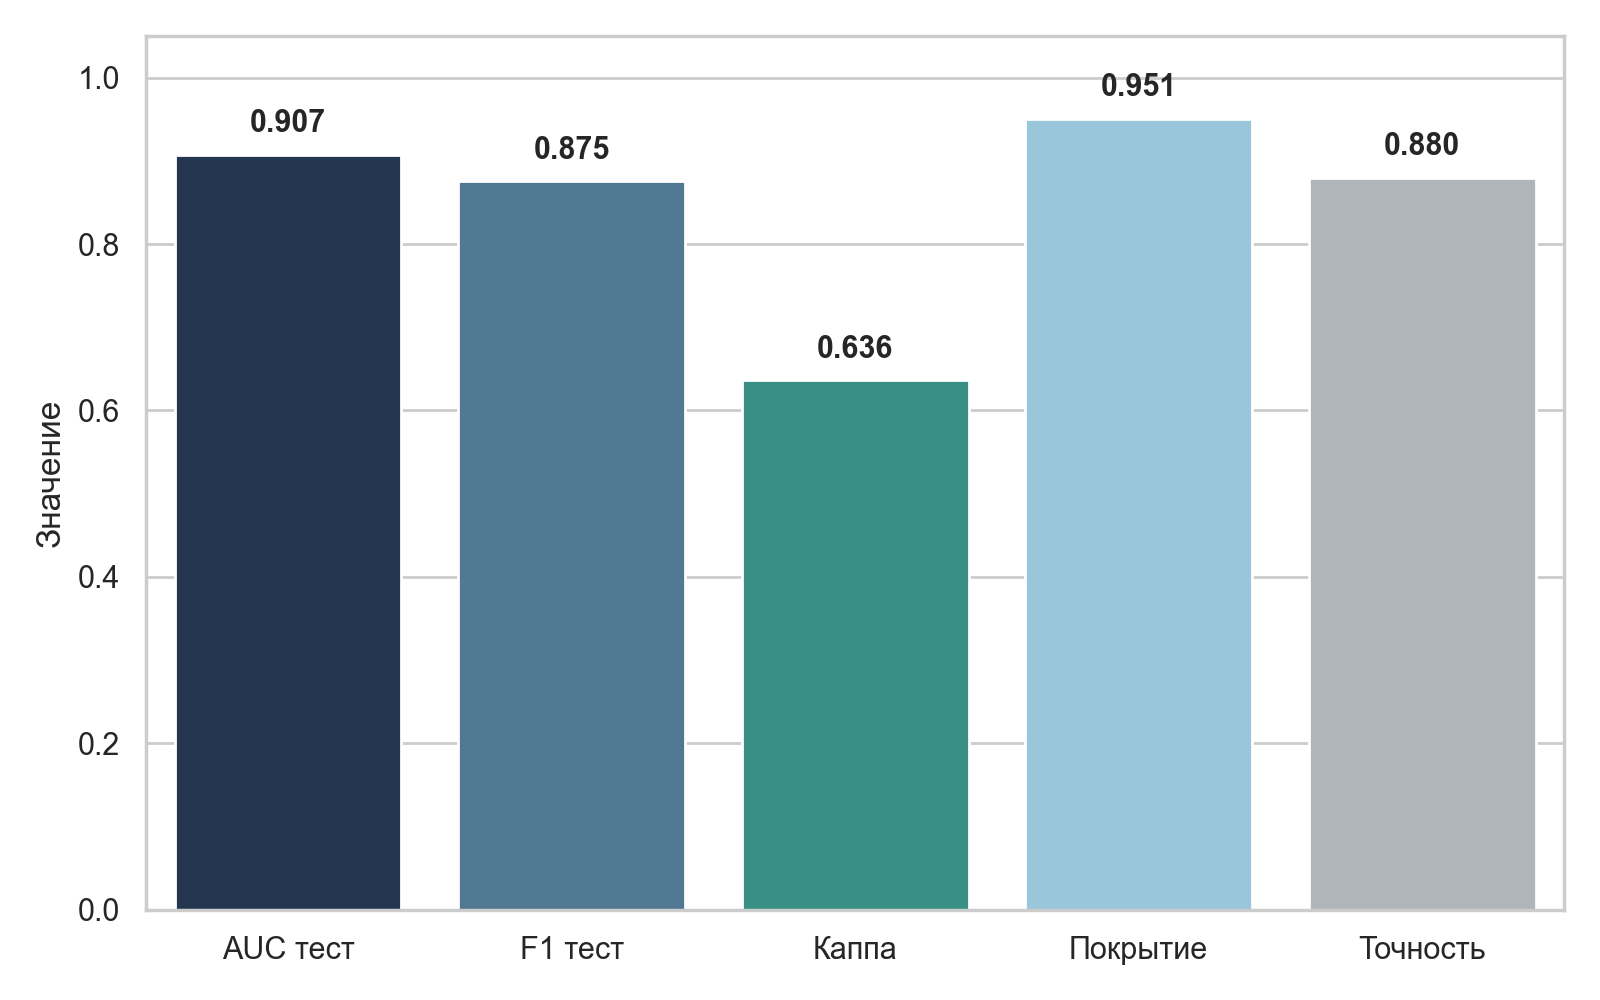
\includegraphics[width=0.88\textwidth]{judge_dashboard.png}
\caption{Компактная агрегированная сводка метрик качества модели-судьи.}
\label{fig:app-judge-dashboard}
\end{figure}

\begin{figure}[htbp]
\centering
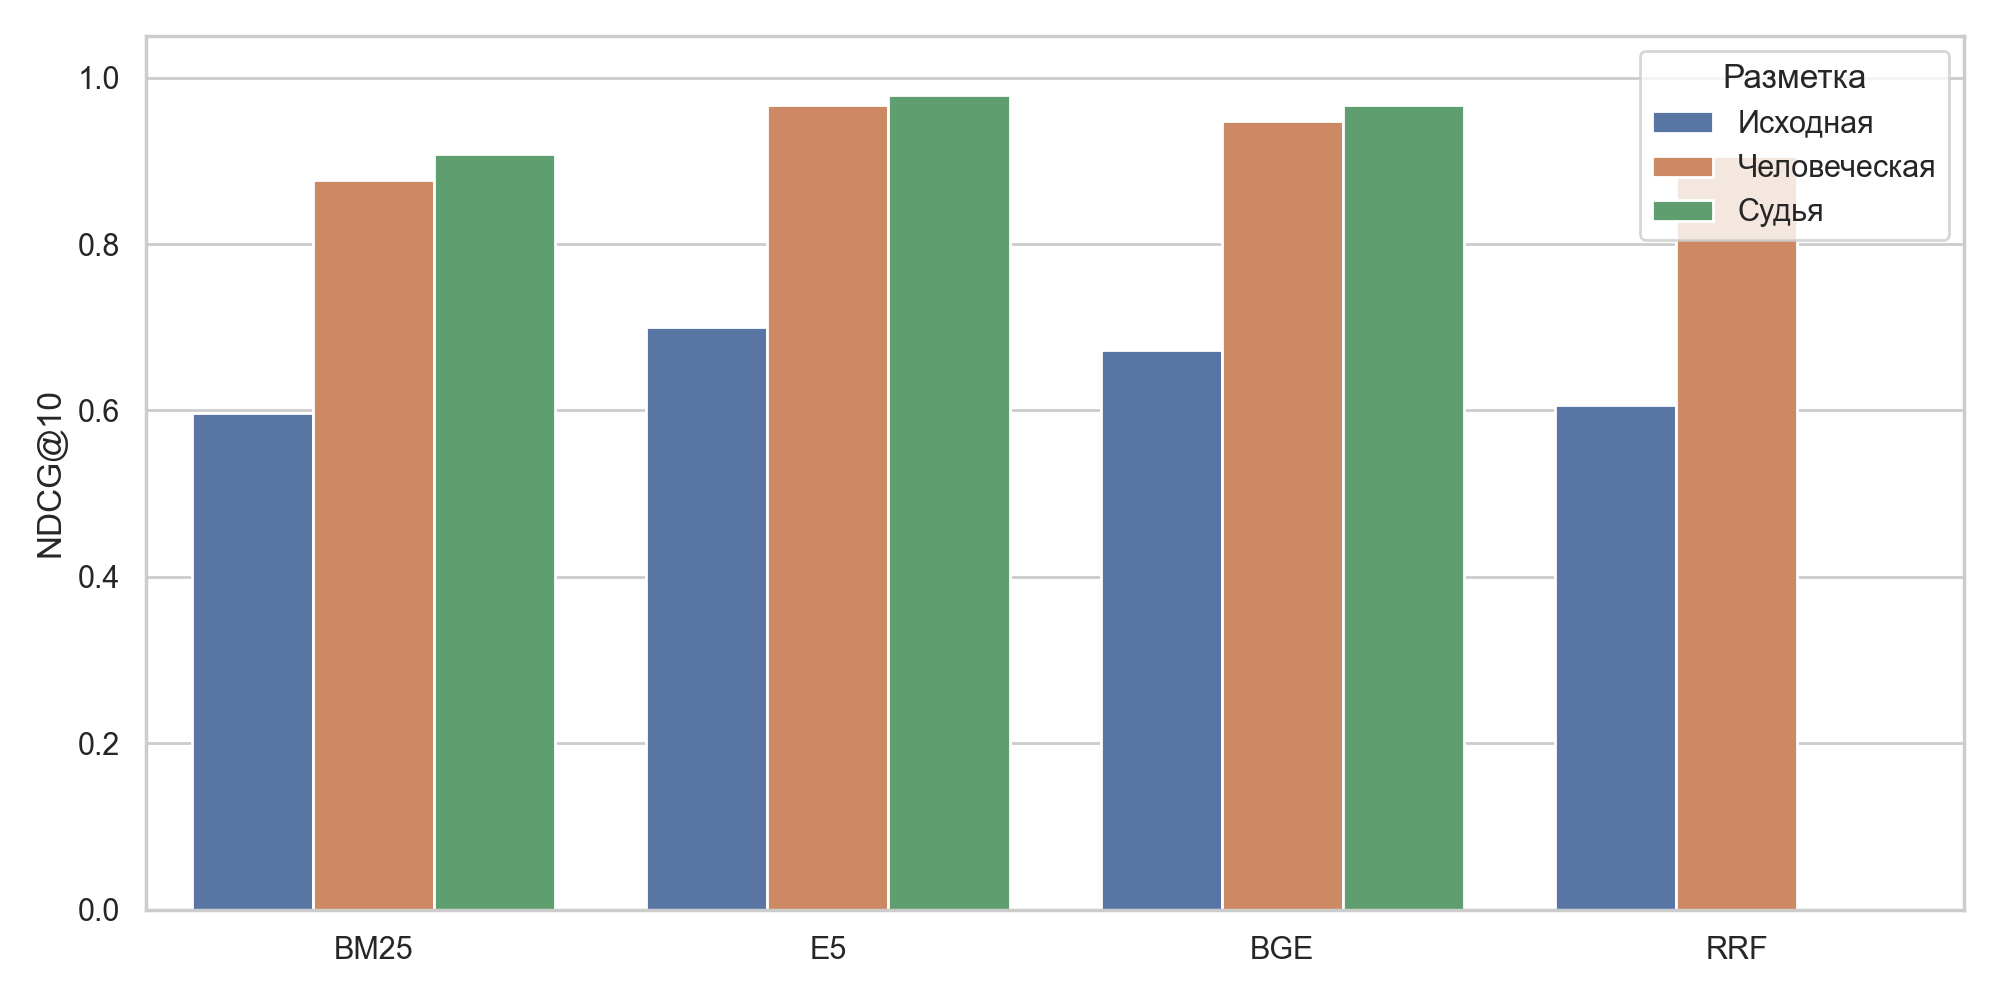
\includegraphics[width=0.90\textwidth]{manual_ndcg_comparison.png}
\caption{Сопоставление исходной ручной разметки, дополнительной человеческой разметки и автоматической разметки модели-судьи для основных моделей.}
\label{fig:app-manual}
\end{figure}

\begin{figure}[htbp]
\centering
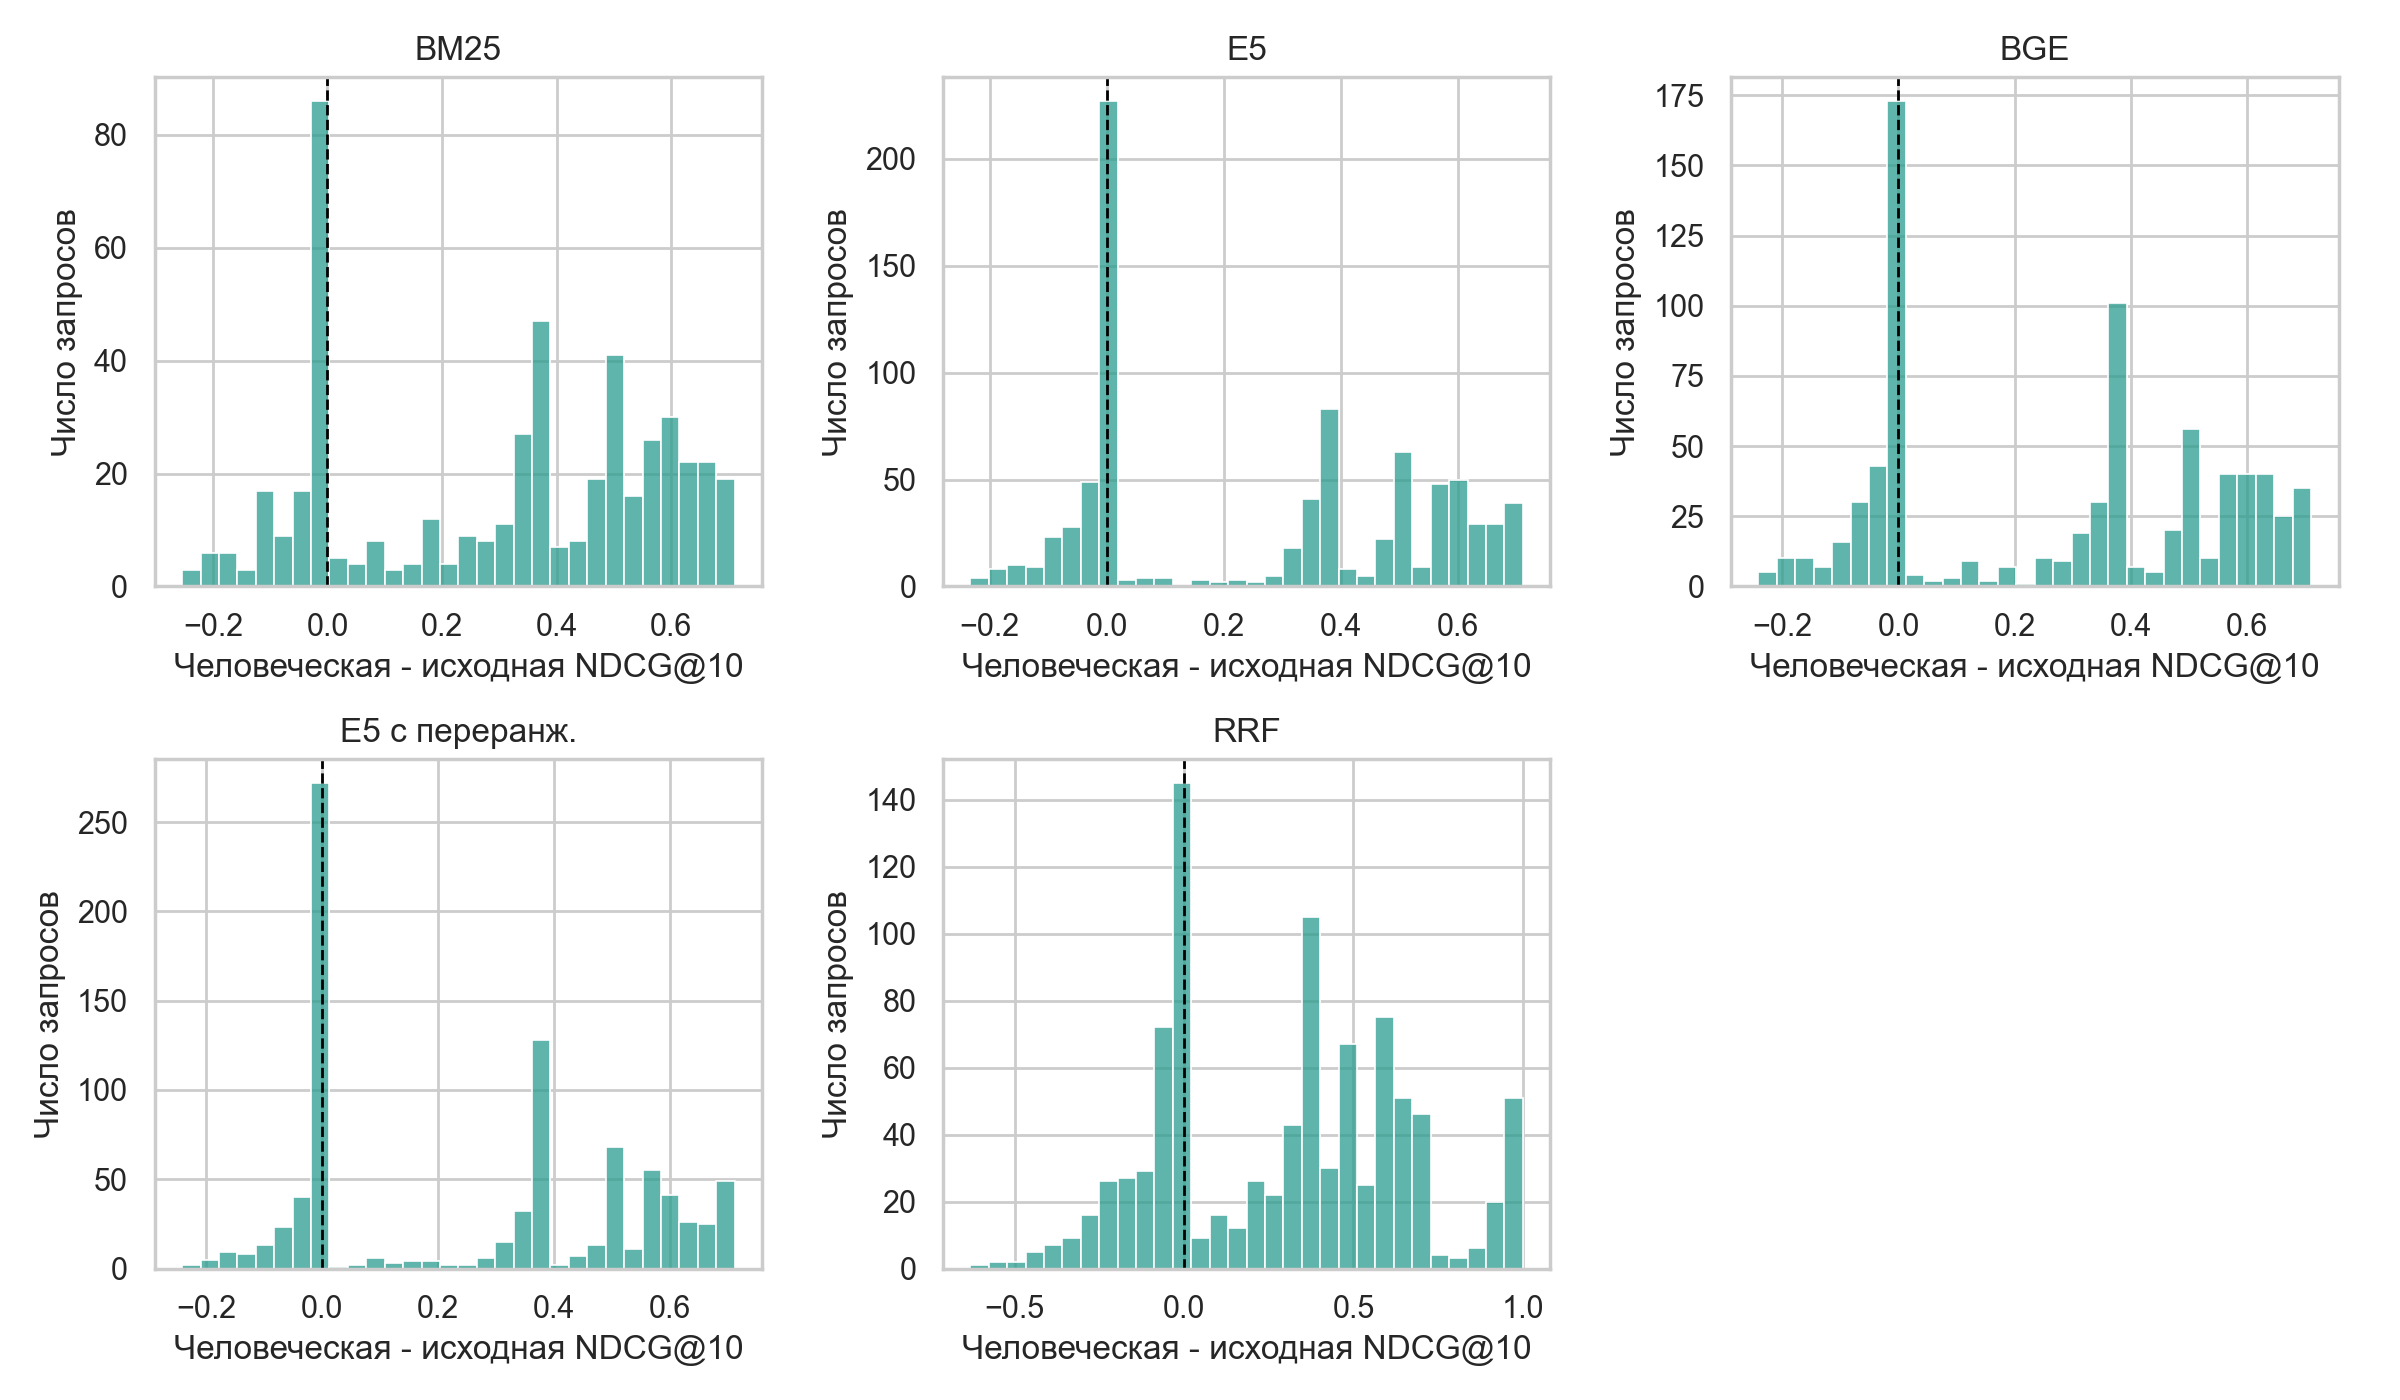
\includegraphics[width=0.90\textwidth]{manual_delta_histograms.png}
\caption{Распределения $\Delta$NDCG@10 по запросам при переходе от исходной разметки к дополнительной человеческой разметке.}
\label{fig:app-delta}
\end{figure}

\begin{figure}[htbp]
\centering
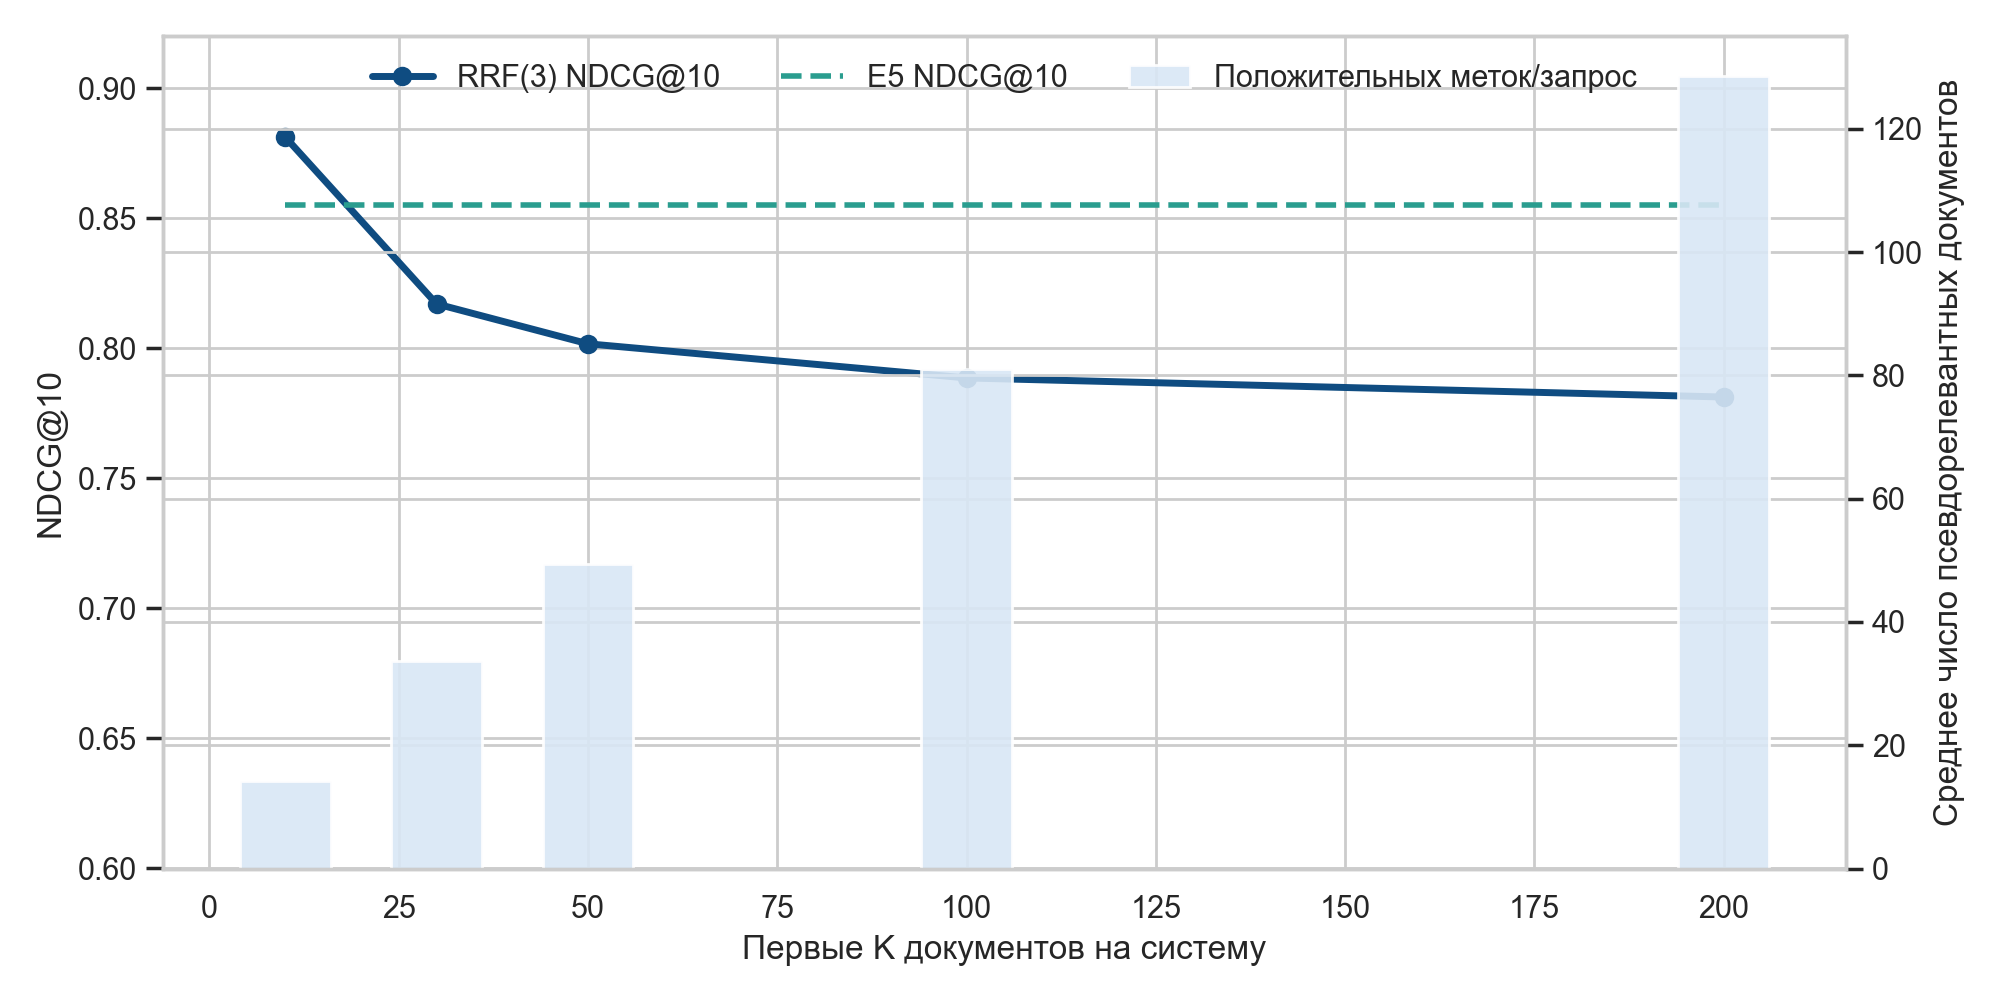
\includegraphics[width=0.88\textwidth]{rrf_sensitivity_dual_axis.png}
\caption{Альтернативная визуализация поведения RRF в полном протоколе с двумя вертикальными осями.}
\label{fig:app-rrf-dual}
\end{figure}

\begin{figure}[htbp]
\centering
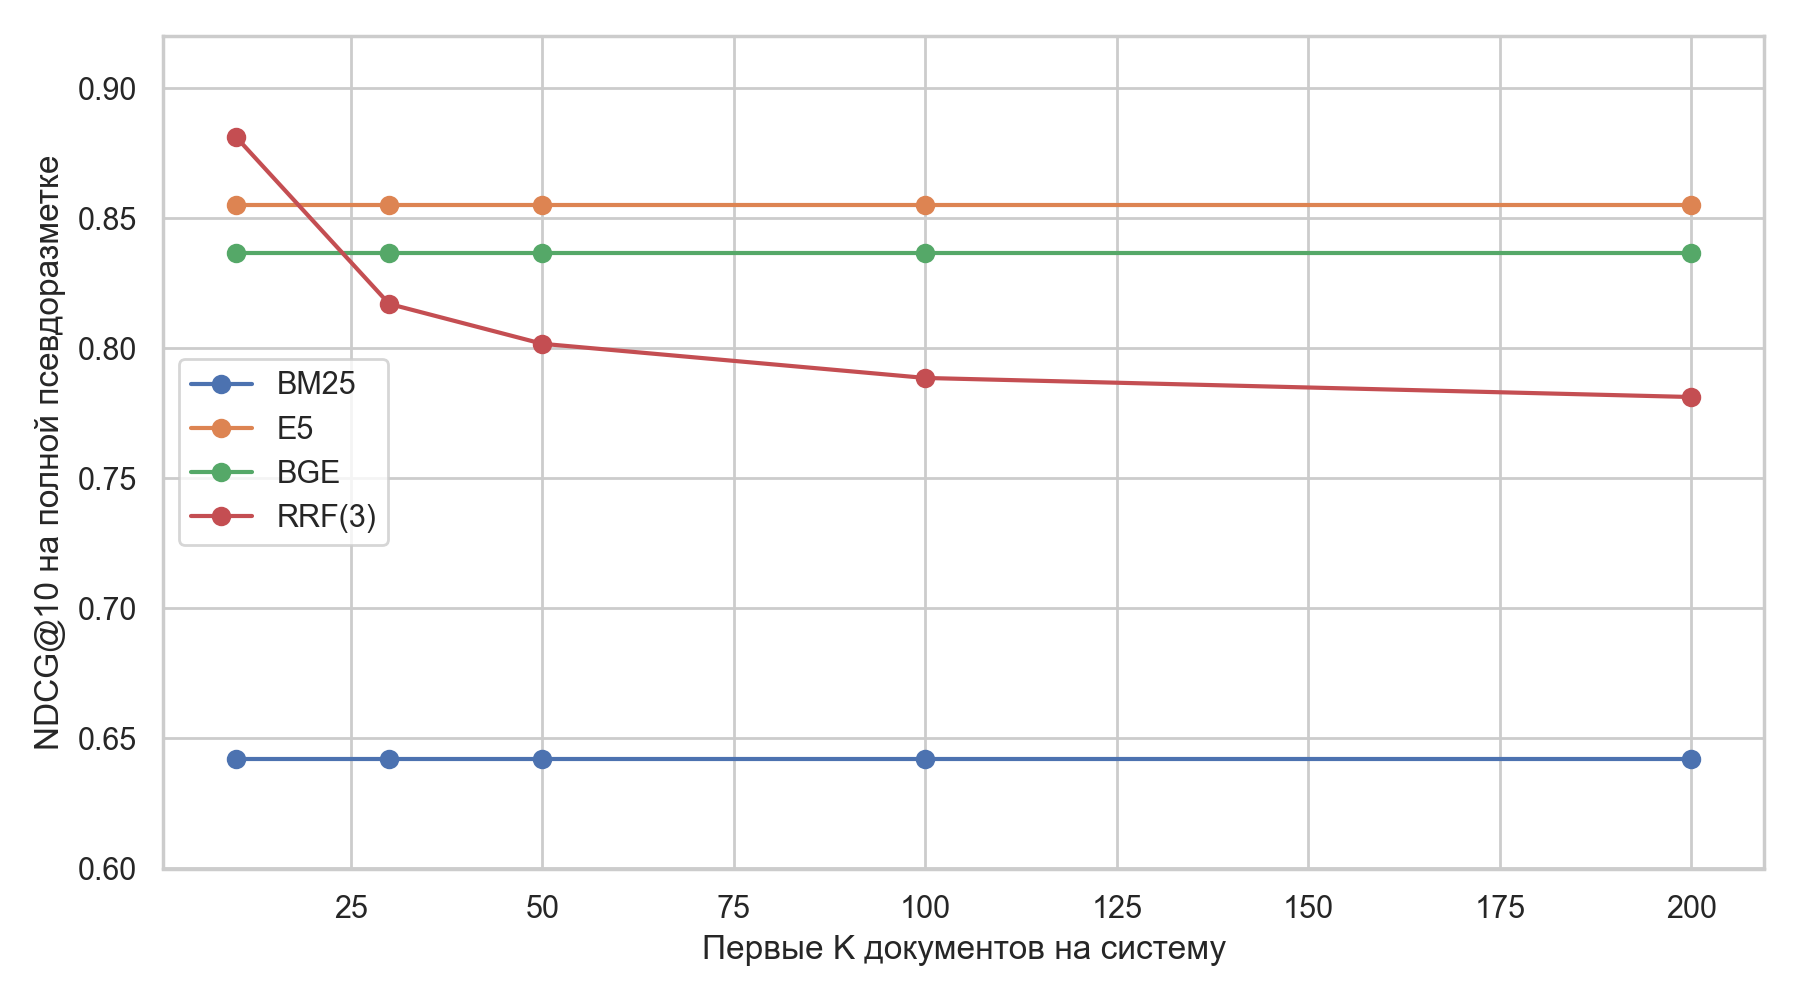
\includegraphics[width=0.90\textwidth]{fullset_rrf_by_pool.png}
\caption{NDCG@10 на псевдоразметке полного набора при различных размерах объединённого пула кандидатов.}
\label{fig:app-pool}
\end{figure}

\begin{figure}[htbp]
\centering
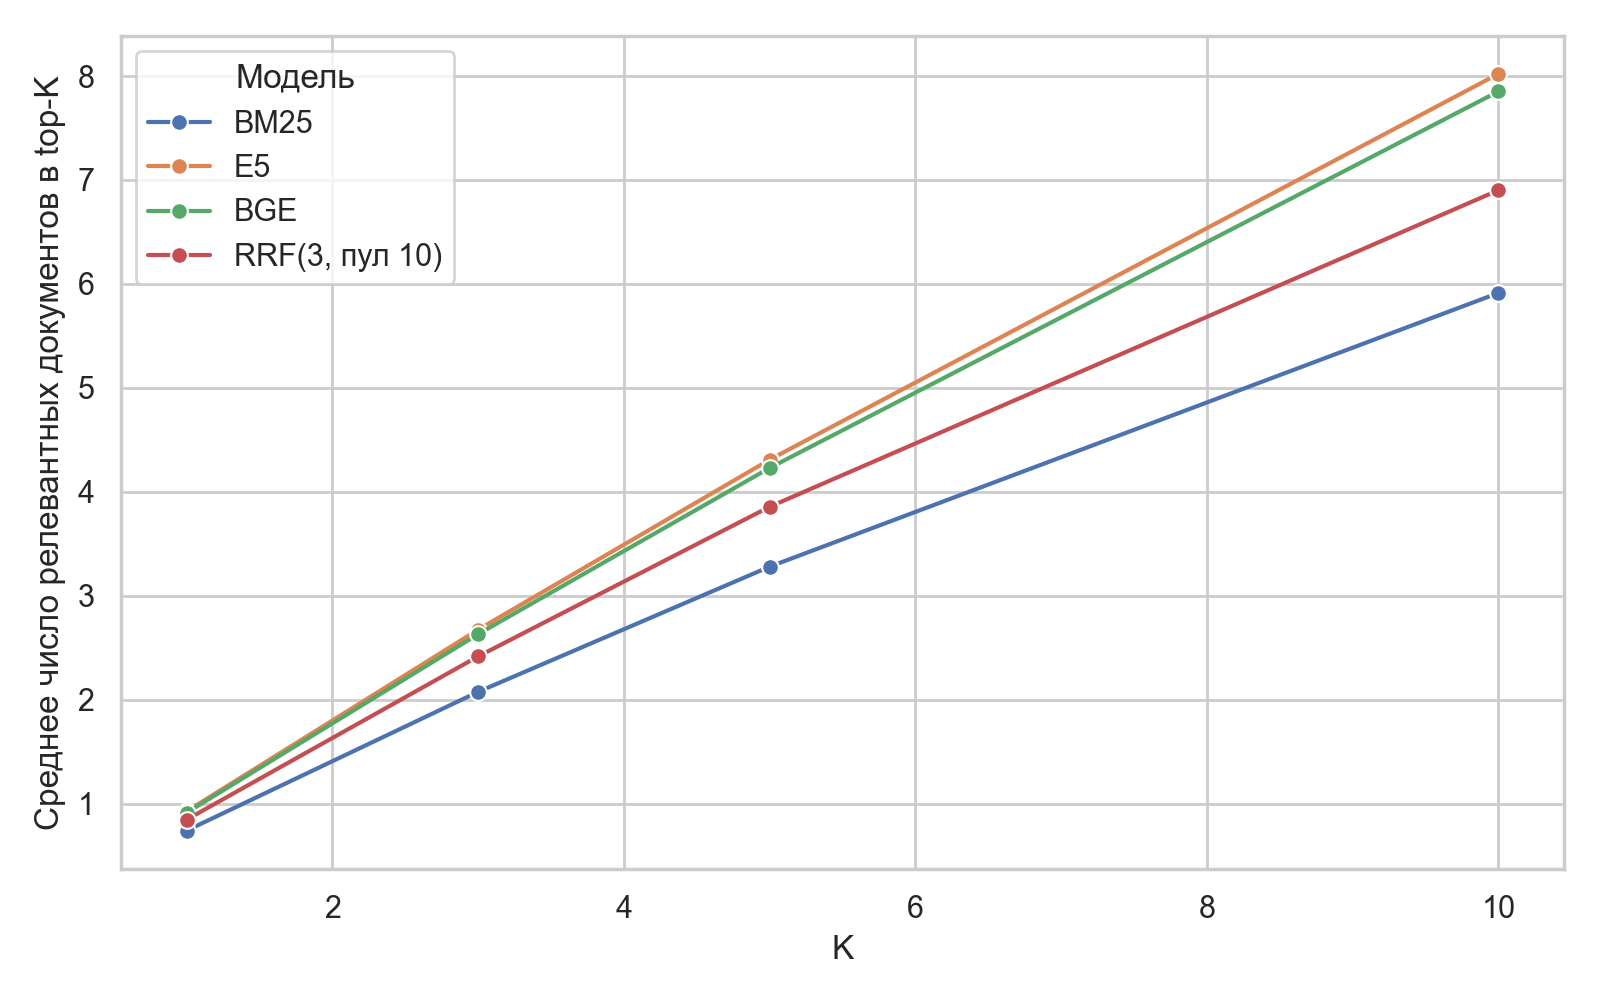
\includegraphics[width=0.90\textwidth]{full_rel_at_k.png}
\caption{Среднее число релевантных документов среди первых $K$ позиций на псевдоразметке полного набора.}
\label{fig:app-relk}
\end{figure}

\begin{figure}[htbp]
\centering
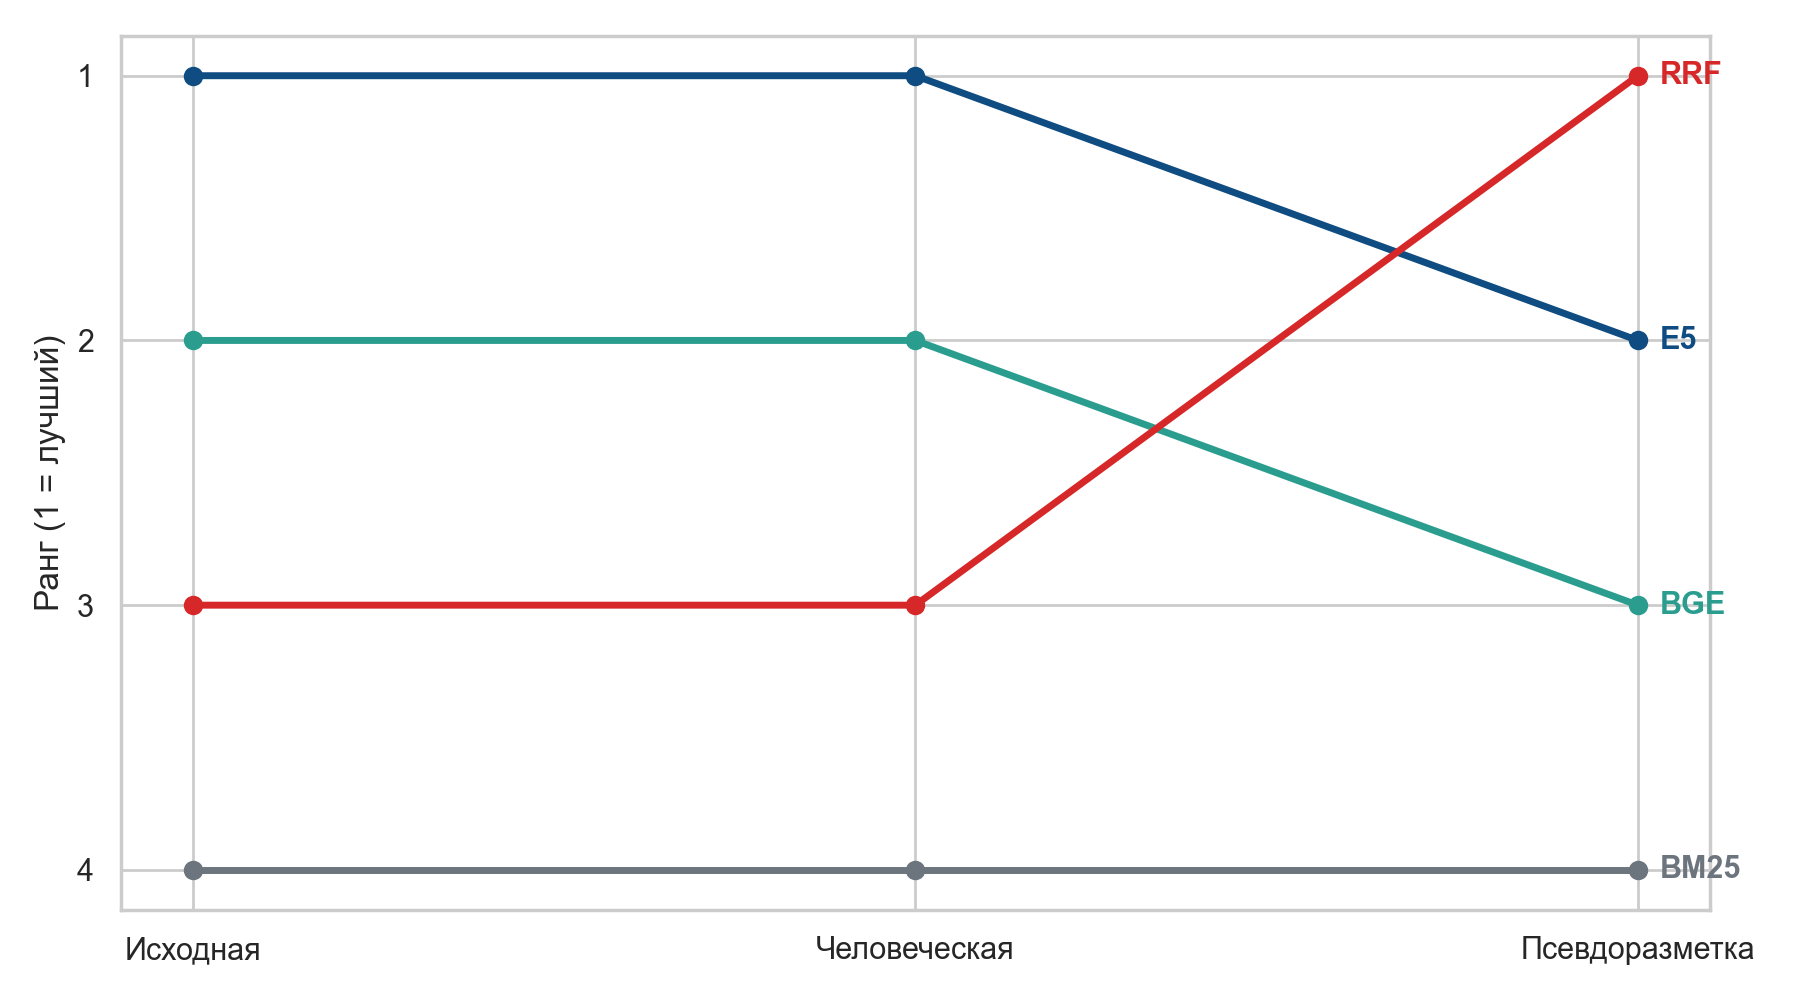
\includegraphics[width=0.90\textwidth]{model_ranking_shift.png}
\caption{Изменение рангового порядка моделей между исходной разметкой, дополнительной человеческой разметкой и псевдоразметкой полного набора.}
\label{fig:app-rank}
\end{figure}

\end{document}
